\documentclass{article}

% Zach del Rosario's LaTeX macros (zdelrosario@outlook.com)
% Inspired by Paul Constantine, Art Owen
% Thanks to David Carlisle for writing the numdef package,
%    which makes the fraction definitions possible!

% Use % Zach del Rosario's LaTeX macros (zdelrosario@outlook.com)
% Inspired by Paul Constantine, Art Owen
% Thanks to David Carlisle for writing the numdef package,
%    which makes the fraction definitions possible!

% Use % Zach del Rosario's LaTeX macros (zdelrosario@outlook.com)
% Inspired by Paul Constantine, Art Owen
% Thanks to David Carlisle for writing the numdef package,
%    which makes the fraction definitions possible!

% Use \input{zachs_macros} in preamble of a latex document

% --------------------------------------------------
% Use some package dependencies
% --------------------------------------------------
\usepackage{amsmath}  % for \boldsymbol, etc.
\usepackage{amsfonts} % for \mathbb, etc.
\usepackage{scalerel,stackengine} % for \reallywidehat{}
\usepackage{graphicx} % for \includegraphics
\usepackage{caption}  % for captioning
\usepackage{mathtools}% for \ceil and \floor
\usepackage{forest}   % for forest environment

% --------------------------------------------------
% Figures and tables
% --------------------------------------------------
% Could use as-is; better for pattern matching

% Image Macro: \img{filename}{caption}
\newcommand{\img}[2]{
	\begin{figure}[H]
	\centering
	\includegraphics[width=0.6\textwidth]{../images/#1}   % first argument is the file
	\caption{#2}                  % second argument is caption
	\label{fig:#1}                % generate label from first argument
	\end{figure} }

% Double Image Macro: \img{file1}{file2}{caption1}{caption2}
\newcommand{\imgtwo}[4]{
	\begin{figure}
	\centering
	\begin{minipage}{.5\textwidth}
		\centering
		\includegraphics[width=0.9\linewidth]{../images/#1}
		\captionof{figure}{#3}
		\label{fig:#1}
	\end{minipage}%
	\begin{minipage}{.5\textwidth}
		\centering
		\includegraphics[width=0.9\linewidth]{../images/#2}
		\captionof{figure}{#4}
		\label{fig:#2}
	\end{minipage}
	\end{figure}
}

% Table Macro: \tab{filename}{caption}
\newcommand{\tab}[2]{
	\begin{table}[H]
	\centering
	\input{#1} 	% first argument is filename
	\caption{#2} 			% second argument is caption
	\label{tab:#1} 			% generate label from filename
	\end{table}
}

% --------------------------------------------------
% Common sets
% --------------------------------------------------
% Lovingly ripped from Art Owen
\def\reals{\mathbb{R}} % Real number symbol
\def\integers{\mathbb{Z}} % Integer symbol
\def\rationals{\mathbb{Q}} % Rational numbers
\def\naturals{\mathbb{N}} % Natural numbers
\def\complex{\mathbb{C}} % Complex numbers
% With exponent
\def\R#1{\mathbb{R}^{#1}}
\def\Z#1{\mathbb{Z}^{#1}}
\def\Q#1{\mathbb{Q}^{#1}}
\def\N#1{\mathbb{N}^{#1}}
\def\C#1{\mathbb{C}^{#1}}

% --------------------------------------------------
% Vectors and Matrices
% --------------------------------------------------
% Transpose symbol
\newcommand{\T}{\top}
% Vector symbol macros
\newcommand{\vsym}[1]{\boldsymbol{#1}}
\def\v#1{\vsym{#1}} % \v{x} for vector symbol
% Quick letter vectors
\newcommand{\va}{\boldsymbol{a}}
\newcommand{\vb}{\boldsymbol{b}}
\newcommand{\vc}{\boldsymbol{c}}
\newcommand{\vd}{\boldsymbol{d}}
\newcommand{\ve}{\boldsymbol{e}}
\newcommand{\vf}{\boldsymbol{f}}
\newcommand{\vg}{\boldsymbol{g}}
\newcommand{\vh}{\boldsymbol{h}}
\newcommand{\vi}{\boldsymbol{i}}
\newcommand{\vj}{\boldsymbol{j}}
\newcommand{\vk}{\boldsymbol{k}}
\newcommand{\vl}{\boldsymbol{l}}
\newcommand{\vm}{\boldsymbol{m}}
\newcommand{\vn}{\boldsymbol{n}}
\newcommand{\vo}{\boldsymbol{o}}
\newcommand{\vp}{\boldsymbol{p}}
\newcommand{\vq}{\boldsymbol{q}}
\newcommand{\vr}{\boldsymbol{r}}
\newcommand{\vs}{\boldsymbol{s}}
\newcommand{\vt}{\boldsymbol{t}}
\newcommand{\vu}{\boldsymbol{u}}
\newcommand{\vv}{\boldsymbol{v}}
\newcommand{\vw}{\boldsymbol{w}}
\newcommand{\vx}{\boldsymbol{x}}
\newcommand{\vy}{\boldsymbol{y}}
\newcommand{\vz}{\boldsymbol{z}}

% Tilde shortcut
\newcommand{\tl}[1]{\tilde{#1}}
% Vector symbol + tilde macros
\newcommand{\vta}{\tilde{\boldsymbol{a}}}
\newcommand{\vtb}{\tilde{\boldsymbol{b}}}
\newcommand{\vtc}{\tilde{\boldsymbol{c}}}
\newcommand{\vtd}{\tilde{\boldsymbol{d}}}
\newcommand{\vte}{\tilde{\boldsymbol{e}}}
\newcommand{\vtf}{\tilde{\boldsymbol{f}}}
\newcommand{\vtg}{\tilde{\boldsymbol{g}}}
\newcommand{\vth}{\tilde{\boldsymbol{h}}}
\newcommand{\vti}{\tilde{\boldsymbol{i}}}
\newcommand{\vtj}{\tilde{\boldsymbol{j}}}
\newcommand{\vtk}{\tilde{\boldsymbol{k}}}
\newcommand{\vtl}{\tilde{\boldsymbol{l}}}
\newcommand{\vtm}{\tilde{\boldsymbol{m}}}
\newcommand{\vtn}{\tilde{\boldsymbol{n}}}
\newcommand{\vto}{\tilde{\boldsymbol{o}}}
\newcommand{\vtp}{\tilde{\boldsymbol{p}}}
\newcommand{\vtq}{\tilde{\boldsymbol{q}}}
\newcommand{\vtr}{\tilde{\boldsymbol{r}}}
\newcommand{\vts}{\tilde{\boldsymbol{s}}}
\newcommand{\vtt}{\tilde{\boldsymbol{t}}}
\newcommand{\vtu}{\tilde{\boldsymbol{u}}}
\newcommand{\vtv}{\tilde{\boldsymbol{v}}}
\newcommand{\vtw}{\tilde{\boldsymbol{w}}}
\newcommand{\vtx}{\tilde{\boldsymbol{x}}}
\newcommand{\vty}{\tilde{\boldsymbol{y}}}
\newcommand{\vtz}{\tilde{\boldsymbol{z}}}

% Vector symbol + hat macros
\newcommand{\vha}{\hat{\boldsymbol{a}}}
\newcommand{\vhb}{\hat{\boldsymbol{b}}}
\newcommand{\vhc}{\hat{\boldsymbol{c}}}
\newcommand{\vhd}{\hat{\boldsymbol{d}}}
\newcommand{\vhe}{\hat{\boldsymbol{e}}}
\newcommand{\vhf}{\hat{\boldsymbol{f}}}
\newcommand{\vhg}{\hat{\boldsymbol{g}}}
\newcommand{\vhh}{\hat{\boldsymbol{h}}}
\newcommand{\vhi}{\hat{\boldsymbol{i}}}
\newcommand{\vhj}{\hat{\boldsymbol{j}}}
\newcommand{\vhk}{\hat{\boldsymbol{k}}}
\newcommand{\vhl}{\hat{\boldsymbol{l}}}
\newcommand{\vhm}{\hat{\boldsymbol{m}}}
\newcommand{\vhn}{\hat{\boldsymbol{n}}}
\newcommand{\vho}{\hat{\boldsymbol{o}}}
\newcommand{\vhp}{\hat{\boldsymbol{p}}}
\newcommand{\vhq}{\hat{\boldsymbol{q}}}
\newcommand{\vhr}{\hat{\boldsymbol{r}}}
\newcommand{\vhs}{\hat{\boldsymbol{s}}}
\newcommand{\vht}{\hat{\boldsymbol{t}}}
\newcommand{\vhu}{\hat{\boldsymbol{u}}}
\newcommand{\vhv}{\hat{\boldsymbol{v}}}
\newcommand{\vhw}{\hat{\boldsymbol{w}}}
\newcommand{\vhx}{\hat{\boldsymbol{x}}}
\newcommand{\vhy}{\hat{\boldsymbol{y}}}
\newcommand{\vhz}{\hat{\boldsymbol{z}}}

% Matrix symbol
\newcommand{\msym}[1]{\boldsymbol{#1}}
\def\m#1{\msym{#1}} % short-shortcut

\newcommand{\mA}{\boldsymbol{A}}
\newcommand{\mB}{\boldsymbol{B}}
\newcommand{\mC}{\boldsymbol{C}}
\newcommand{\mD}{\boldsymbol{D}}
\newcommand{\mE}{\boldsymbol{E}}
\newcommand{\mF}{\boldsymbol{F}}
\newcommand{\mG}{\boldsymbol{G}}
\newcommand{\mH}{\boldsymbol{H}}
\newcommand{\mI}{\boldsymbol{I}}
\newcommand{\mJ}{\boldsymbol{J}}
\newcommand{\mK}{\boldsymbol{K}}
\newcommand{\mL}{\boldsymbol{L}}
\newcommand{\mM}{\boldsymbol{M}}
\newcommand{\mN}{\boldsymbol{N}}
\newcommand{\mO}{\boldsymbol{O}}
\newcommand{\mP}{\boldsymbol{P}}
\newcommand{\mQ}{\boldsymbol{Q}}
\newcommand{\mR}{\boldsymbol{R}}
\newcommand{\mS}{\boldsymbol{S}}
\newcommand{\mT}{\boldsymbol{T}}
\newcommand{\mU}{\boldsymbol{U}}
\newcommand{\mV}{\boldsymbol{V}}
\newcommand{\mW}{\boldsymbol{W}}
\newcommand{\mX}{\boldsymbol{X}}
\newcommand{\mY}{\boldsymbol{Y}}
\newcommand{\mZ}{\boldsymbol{Z}}

% Tilde over letter
\newcommand{\tla}{\tilde{a}}
\newcommand{\tlb}{\tilde{b}}
\newcommand{\tlc}{\tilde{c}}
\newcommand{\tld}{\tilde{d}}
\newcommand{\tle}{\tilde{e}}
\newcommand{\tlf}{\tilde{f}}
\newcommand{\tlg}{\tilde{g}}
\newcommand{\tlh}{\tilde{h}}
\newcommand{\tli}{\tilde{i}}
\newcommand{\tlj}{\tilde{j}}
\newcommand{\tlk}{\tilde{k}}
\newcommand{\tll}{\tilde{l}}
\newcommand{\tlm}{\tilde{m}}
\newcommand{\tln}{\tilde{n}}
\newcommand{\tlo}{\tilde{o}}
\newcommand{\tlp}{\tilde{p}}
\newcommand{\tlq}{\tilde{q}}
\newcommand{\tlr}{\tilde{r}}
\newcommand{\tls}{\tilde{s}}
\newcommand{\tlt}{\tilde{t}}
\newcommand{\tlu}{\tilde{u}}
\newcommand{\tlv}{\tilde{v}}
\newcommand{\tlw}{\tilde{w}}
\newcommand{\tlx}{\tilde{x}}
\newcommand{\tly}{\tilde{y}}
\newcommand{\tlz}{\tilde{z}}

% Caligraphic symbol
\def\c#1{\mathcal{#1}} % short-shortcut

\newcommand{\cA}{\mathcal{A}}
\newcommand{\cB}{\mathcal{B}}
\newcommand{\cC}{\mathcal{C}}
\newcommand{\cD}{\mathcal{D}}
\newcommand{\cE}{\mathcal{E}}
\newcommand{\cF}{\mathcal{F}}
\newcommand{\cG}{\mathcal{G}}
\newcommand{\cH}{\mathcal{H}}
\newcommand{\cI}{\mathcal{I}}
\newcommand{\cJ}{\mathcal{J}}
\newcommand{\cK}{\mathcal{K}}
\newcommand{\cL}{\mathcal{L}}
\newcommand{\cM}{\mathcal{M}}
\newcommand{\cN}{\mathcal{N}}
\newcommand{\cO}{\mathcal{O}}
\newcommand{\cP}{\mathcal{P}}
\newcommand{\cQ}{\mathcal{Q}}
\newcommand{\cR}{\mathcal{R}}
\newcommand{\cS}{\mathcal{S}}
\newcommand{\cT}{\mathcal{T}}
\newcommand{\cU}{\mathcal{U}}
\newcommand{\cV}{\mathcal{V}}
\newcommand{\cW}{\mathcal{W}}
\newcommand{\cX}{\mathcal{X}}
\newcommand{\cY}{\mathcal{Y}}
\newcommand{\cZ}{\mathcal{Z}}
% --------------------------------------------------
% Common probability symbols
% --------------------------------------------------
% Lovingly ripped from Art Owen
\newcommand{\mrm}{\mathrm}
\def\E{\mathbb{E}} % Expectation symbol
\def\Earg#1{\E\left[{#1}\right]}
\def\Esubarg#1#2{\E_{#1}\left[{#2}\right]}
\def\P{\mathbb{P}} % Probability symbol
\def\Parg#1{\P\left({#1}\right)}
\def\Psubarg#1#2{\P_{#1}\left[{#2}\right]}
\def\Cov{\mrm{Cov}} % Covariance symbol
\def\Covarg#1{\Cov\left[{#1}\right]}
\def\Covsubarg#1#2{\Cov_{#1}\left[{#2}\right]}
\newcommand{\family}{\mathcal{P}} % probability family / statistical model
\newcommand{\iid}{\stackrel{\mathrm{iid}}{\sim}}
\newcommand{\ind}{\stackrel{\mathrm{ind}}{\sim}}
\def\V{\mathrm{V}} % Variance symbol
\newcommand{\dN}{\mathcal{N}} % Normal distribution

% --------------------------------------------------
% Misc
% --------------------------------------------------
% Indicator function
\def\i1{\mathbb{1}}

% Angle bracket average
\newcommand{\avg}[1]{\left\langle#1\right\rangle}

% Markless footnote
% https://tex.stackexchange.com/questions/30720/footnote-without-a-marker
\newcommand\blfootnote[1]{%
  \begingroup
  \renewcommand\thefootnote{}\footnote{#1}%
  \addtocounter{footnote}{-1}%
  \endgroup
}

% Floor and ceiling
% http://tex.stackexchange.com/questions/118173/how-to-write-ceil-and-floor-in-latex
\DeclarePairedDelimiter\ceil{\lceil}{\rceil}
\DeclarePairedDelimiter\floor{\lfloor}{\rfloor}

% Comical & useful reallywidehat
\stackMath
\newcommand\reallywidehat[1]{%
\savestack{\tmpbox}{\stretchto{%
  \scaleto{%
    \scalerel*[\widthof{\ensuremath{#1}}]{\kern-.6pt\bigwedge\kern-.6pt}%
    {\rule[-\textheight/2]{1ex}{\textheight}}%WIDTH-LIMITED BIG WEDGE
  }{\textheight}%
}{0.5ex}}%
\stackon[1pt]{#1}{\tmpbox}%
}

% Comical & useful reallywideparen
\newcommand\reallywideparen[1]{%
\begin{array}{c}
\stretchto{
  \scaleto{
    \scalerel*[\widthof{#1}]{\frown}
    {\rule[-\textheight/2]{1ex}{\textheight}} %WIDTH-LIMITED BIG WEDGE
  }{1.25\textheight} % THIS STRETCHES THE WEDGE A LITTLE EXTRA WIDE
}{0.5ex}\\           % THIS SQUEEZES THE WEDGE TO 0.5ex HEIGHT
#1\\                   % THIS STACKS THE WEDGE ATOP THE ARGUMENT
\rule{0ex}{.01ex}
\end{array}
}
% Useful for debugging; prints to document whether command has been defined already
% Via: http://tex.stackexchange.com/questions/30483/how-can-i-check-in-latex-or-plain-tex-whether-a-command-exists-by-name
\newcommand{\checkfor}[1]{%
  \ifcsname#1\endcsname%
    ... command '#1' exists ...%
  \else%
    ... command '#1' does not exist ...%
  \fi%
}

% Use a forest environment to depict a directory tree
% https://tex.stackexchange.com/questions/5073/making-a-simple-directory-tree
\newcommand{\ftree}[1]{%
\begin{forest}
for tree={
    font=\ttfamily,
    grow'=0,
    child anchor=west,
    parent anchor=south,
    anchor=west,
    calign=first,
    edge path={
      \noexpand\path [draw, \forestoption{edge}]
      (!u.south west) +(7.5pt,0) |- node[fill,inner sep=1.25pt] {} (.child anchor)\forestoption{edge label};
    },
    before typesetting nodes={
      if n=1
        {insert before={[,phantom]}}
        {}
    },
    fit=band,
    before computing xy={l=15pt},
  }%
  #1%
\end{forest}
}

% --------------------------------------------------
% Fractions
% --------------------------------------------------
\usepackage{numdef}   % prefixing with \num allows numbers at end of \newcommand name
\num\newcommand{\f12}{\frac{1}{2}}
\num\newcommand{\f13}{\frac{1}{3}}
\num\newcommand{\f14}{\frac{1}{4}}
\num\newcommand{\f15}{\frac{1}{5}}
\num\newcommand{\f16}{\frac{1}{6}}
\num\newcommand{\f17}{\frac{1}{7}}
\num\newcommand{\f18}{\frac{1}{8}}
\num\newcommand{\f19}{\frac{1}{9}}

\num\newcommand{\f22}{\frac{2}{2}}
\num\newcommand{\f23}{\frac{2}{3}}
\num\newcommand{\f24}{\frac{2}{4}}
\num\newcommand{\f25}{\frac{2}{5}}
\num\newcommand{\f26}{\frac{2}{6}}
\num\newcommand{\f27}{\frac{2}{7}}
\num\newcommand{\f28}{\frac{2}{8}}
\num\newcommand{\f29}{\frac{2}{9}}

\num\newcommand{\f32}{\frac{3}{2}}
\num\newcommand{\f33}{\frac{3}{3}}
\num\newcommand{\f34}{\frac{3}{4}}
\num\newcommand{\f35}{\frac{3}{5}}
\num\newcommand{\f36}{\frac{3}{6}}
\num\newcommand{\f37}{\frac{3}{7}}
\num\newcommand{\f38}{\frac{3}{8}}
\num\newcommand{\f39}{\frac{3}{9}}

\num\newcommand{\f42}{\frac{4}{2}}
\num\newcommand{\f43}{\frac{4}{3}}
\num\newcommand{\f44}{\frac{4}{4}}
\num\newcommand{\f45}{\frac{4}{5}}
\num\newcommand{\f46}{\frac{4}{6}}
\num\newcommand{\f47}{\frac{4}{7}}
\num\newcommand{\f48}{\frac{4}{8}}
\num\newcommand{\f49}{\frac{4}{9}}

\num\newcommand{\f52}{\frac{5}{2}}
\num\newcommand{\f53}{\frac{5}{3}}
\num\newcommand{\f54}{\frac{5}{4}}
\num\newcommand{\f55}{\frac{5}{5}}
\num\newcommand{\f56}{\frac{5}{6}}
\num\newcommand{\f57}{\frac{5}{7}}
\num\newcommand{\f58}{\frac{5}{8}}
\num\newcommand{\f59}{\frac{5}{9}}

\num\newcommand{\f62}{\frac{6}{2}}
\num\newcommand{\f63}{\frac{6}{3}}
\num\newcommand{\f64}{\frac{6}{4}}
\num\newcommand{\f65}{\frac{6}{5}}
\num\newcommand{\f66}{\frac{6}{6}}
\num\newcommand{\f67}{\frac{6}{7}}
\num\newcommand{\f68}{\frac{6}{8}}
\num\newcommand{\f69}{\frac{6}{9}}

\num\newcommand{\f72}{\frac{7}{2}}
\num\newcommand{\f73}{\frac{7}{3}}
\num\newcommand{\f74}{\frac{7}{4}}
\num\newcommand{\f75}{\frac{7}{5}}
\num\newcommand{\f76}{\frac{7}{6}}
\num\newcommand{\f77}{\frac{7}{7}}
\num\newcommand{\f78}{\frac{7}{8}}
\num\newcommand{\f79}{\frac{7}{9}}

\num\newcommand{\f82}{\frac{8}{2}}
\num\newcommand{\f83}{\frac{8}{3}}
\num\newcommand{\f84}{\frac{8}{4}}
\num\newcommand{\f85}{\frac{8}{5}}
\num\newcommand{\f86}{\frac{8}{6}}
\num\newcommand{\f87}{\frac{8}{7}}
\num\newcommand{\f88}{\frac{8}{8}}
\num\newcommand{\f89}{\frac{8}{9}}

\num\newcommand{\f92}{\frac{9}{2}}
\num\newcommand{\f93}{\frac{9}{3}}
\num\newcommand{\f94}{\frac{9}{4}}
\num\newcommand{\f95}{\frac{9}{5}}
\num\newcommand{\f96}{\frac{9}{6}}
\num\newcommand{\f97}{\frac{9}{7}}
\num\newcommand{\f98}{\frac{9}{8}}
\num\newcommand{\f99}{\frac{9}{9}}

% --------------------------------------------------
% Cylindrical and Spherical operators
% --------------------------------------------------
% Cylindrical coordinates {r,\phi,z}
\num\newcommand{\cdiv1}[1]{\frac{1}{r}\frac{\partial}{\partial r}(r#1)}
\num\newcommand{\cdiv2}[1]{\frac{1}{r}\frac{\partial}{\partial\phi}(#1)}
\num\newcommand{\cdiv3}[1]{\frac{\partial}{\partial z}(#1)}

%--------------------------------------------------
% matminux
%--------------------------------------------------
% https://tex.stackexchange.com/questions/75545/negative-sign-and-matrix-alignment
\newcommand*{\mm}{%
  \leavevmode
  \hphantom{0}%
  \llap{%
    \settowidth{\dimen0 }{$0$}%
    \resizebox{1.1\dimen0 }{\height}{$-$}%
  }%
}
 in preamble of a latex document

% --------------------------------------------------
% Use some package dependencies
% --------------------------------------------------
\usepackage{amsmath}  % for \boldsymbol, etc.
\usepackage{amsfonts} % for \mathbb, etc.
\usepackage{scalerel,stackengine} % for \reallywidehat{}
\usepackage{graphicx} % for \includegraphics
\usepackage{caption}  % for captioning
\usepackage{mathtools}% for \ceil and \floor
\usepackage{forest}   % for forest environment

% --------------------------------------------------
% Figures and tables
% --------------------------------------------------
% Could use as-is; better for pattern matching

% Image Macro: \img{filename}{caption}
\newcommand{\img}[2]{
	\begin{figure}[H]
	\centering
	\includegraphics[width=0.6\textwidth]{../images/#1}   % first argument is the file
	\caption{#2}                  % second argument is caption
	\label{fig:#1}                % generate label from first argument
	\end{figure} }

% Double Image Macro: \img{file1}{file2}{caption1}{caption2}
\newcommand{\imgtwo}[4]{
	\begin{figure}
	\centering
	\begin{minipage}{.5\textwidth}
		\centering
		\includegraphics[width=0.9\linewidth]{../images/#1}
		\captionof{figure}{#3}
		\label{fig:#1}
	\end{minipage}%
	\begin{minipage}{.5\textwidth}
		\centering
		\includegraphics[width=0.9\linewidth]{../images/#2}
		\captionof{figure}{#4}
		\label{fig:#2}
	\end{minipage}
	\end{figure}
}

% Table Macro: \tab{filename}{caption}
\newcommand{\tab}[2]{
	\begin{table}[H]
	\centering
	\input{#1} 	% first argument is filename
	\caption{#2} 			% second argument is caption
	\label{tab:#1} 			% generate label from filename
	\end{table}
}

% --------------------------------------------------
% Common sets
% --------------------------------------------------
% Lovingly ripped from Art Owen
\def\reals{\mathbb{R}} % Real number symbol
\def\integers{\mathbb{Z}} % Integer symbol
\def\rationals{\mathbb{Q}} % Rational numbers
\def\naturals{\mathbb{N}} % Natural numbers
\def\complex{\mathbb{C}} % Complex numbers
% With exponent
\def\R#1{\mathbb{R}^{#1}}
\def\Z#1{\mathbb{Z}^{#1}}
\def\Q#1{\mathbb{Q}^{#1}}
\def\N#1{\mathbb{N}^{#1}}
\def\C#1{\mathbb{C}^{#1}}

% --------------------------------------------------
% Vectors and Matrices
% --------------------------------------------------
% Transpose symbol
\newcommand{\T}{\top}
% Vector symbol macros
\newcommand{\vsym}[1]{\boldsymbol{#1}}
\def\v#1{\vsym{#1}} % \v{x} for vector symbol
% Quick letter vectors
\newcommand{\va}{\boldsymbol{a}}
\newcommand{\vb}{\boldsymbol{b}}
\newcommand{\vc}{\boldsymbol{c}}
\newcommand{\vd}{\boldsymbol{d}}
\newcommand{\ve}{\boldsymbol{e}}
\newcommand{\vf}{\boldsymbol{f}}
\newcommand{\vg}{\boldsymbol{g}}
\newcommand{\vh}{\boldsymbol{h}}
\newcommand{\vi}{\boldsymbol{i}}
\newcommand{\vj}{\boldsymbol{j}}
\newcommand{\vk}{\boldsymbol{k}}
\newcommand{\vl}{\boldsymbol{l}}
\newcommand{\vm}{\boldsymbol{m}}
\newcommand{\vn}{\boldsymbol{n}}
\newcommand{\vo}{\boldsymbol{o}}
\newcommand{\vp}{\boldsymbol{p}}
\newcommand{\vq}{\boldsymbol{q}}
\newcommand{\vr}{\boldsymbol{r}}
\newcommand{\vs}{\boldsymbol{s}}
\newcommand{\vt}{\boldsymbol{t}}
\newcommand{\vu}{\boldsymbol{u}}
\newcommand{\vv}{\boldsymbol{v}}
\newcommand{\vw}{\boldsymbol{w}}
\newcommand{\vx}{\boldsymbol{x}}
\newcommand{\vy}{\boldsymbol{y}}
\newcommand{\vz}{\boldsymbol{z}}

% Tilde shortcut
\newcommand{\tl}[1]{\tilde{#1}}
% Vector symbol + tilde macros
\newcommand{\vta}{\tilde{\boldsymbol{a}}}
\newcommand{\vtb}{\tilde{\boldsymbol{b}}}
\newcommand{\vtc}{\tilde{\boldsymbol{c}}}
\newcommand{\vtd}{\tilde{\boldsymbol{d}}}
\newcommand{\vte}{\tilde{\boldsymbol{e}}}
\newcommand{\vtf}{\tilde{\boldsymbol{f}}}
\newcommand{\vtg}{\tilde{\boldsymbol{g}}}
\newcommand{\vth}{\tilde{\boldsymbol{h}}}
\newcommand{\vti}{\tilde{\boldsymbol{i}}}
\newcommand{\vtj}{\tilde{\boldsymbol{j}}}
\newcommand{\vtk}{\tilde{\boldsymbol{k}}}
\newcommand{\vtl}{\tilde{\boldsymbol{l}}}
\newcommand{\vtm}{\tilde{\boldsymbol{m}}}
\newcommand{\vtn}{\tilde{\boldsymbol{n}}}
\newcommand{\vto}{\tilde{\boldsymbol{o}}}
\newcommand{\vtp}{\tilde{\boldsymbol{p}}}
\newcommand{\vtq}{\tilde{\boldsymbol{q}}}
\newcommand{\vtr}{\tilde{\boldsymbol{r}}}
\newcommand{\vts}{\tilde{\boldsymbol{s}}}
\newcommand{\vtt}{\tilde{\boldsymbol{t}}}
\newcommand{\vtu}{\tilde{\boldsymbol{u}}}
\newcommand{\vtv}{\tilde{\boldsymbol{v}}}
\newcommand{\vtw}{\tilde{\boldsymbol{w}}}
\newcommand{\vtx}{\tilde{\boldsymbol{x}}}
\newcommand{\vty}{\tilde{\boldsymbol{y}}}
\newcommand{\vtz}{\tilde{\boldsymbol{z}}}

% Vector symbol + hat macros
\newcommand{\vha}{\hat{\boldsymbol{a}}}
\newcommand{\vhb}{\hat{\boldsymbol{b}}}
\newcommand{\vhc}{\hat{\boldsymbol{c}}}
\newcommand{\vhd}{\hat{\boldsymbol{d}}}
\newcommand{\vhe}{\hat{\boldsymbol{e}}}
\newcommand{\vhf}{\hat{\boldsymbol{f}}}
\newcommand{\vhg}{\hat{\boldsymbol{g}}}
\newcommand{\vhh}{\hat{\boldsymbol{h}}}
\newcommand{\vhi}{\hat{\boldsymbol{i}}}
\newcommand{\vhj}{\hat{\boldsymbol{j}}}
\newcommand{\vhk}{\hat{\boldsymbol{k}}}
\newcommand{\vhl}{\hat{\boldsymbol{l}}}
\newcommand{\vhm}{\hat{\boldsymbol{m}}}
\newcommand{\vhn}{\hat{\boldsymbol{n}}}
\newcommand{\vho}{\hat{\boldsymbol{o}}}
\newcommand{\vhp}{\hat{\boldsymbol{p}}}
\newcommand{\vhq}{\hat{\boldsymbol{q}}}
\newcommand{\vhr}{\hat{\boldsymbol{r}}}
\newcommand{\vhs}{\hat{\boldsymbol{s}}}
\newcommand{\vht}{\hat{\boldsymbol{t}}}
\newcommand{\vhu}{\hat{\boldsymbol{u}}}
\newcommand{\vhv}{\hat{\boldsymbol{v}}}
\newcommand{\vhw}{\hat{\boldsymbol{w}}}
\newcommand{\vhx}{\hat{\boldsymbol{x}}}
\newcommand{\vhy}{\hat{\boldsymbol{y}}}
\newcommand{\vhz}{\hat{\boldsymbol{z}}}

% Matrix symbol
\newcommand{\msym}[1]{\boldsymbol{#1}}
\def\m#1{\msym{#1}} % short-shortcut

\newcommand{\mA}{\boldsymbol{A}}
\newcommand{\mB}{\boldsymbol{B}}
\newcommand{\mC}{\boldsymbol{C}}
\newcommand{\mD}{\boldsymbol{D}}
\newcommand{\mE}{\boldsymbol{E}}
\newcommand{\mF}{\boldsymbol{F}}
\newcommand{\mG}{\boldsymbol{G}}
\newcommand{\mH}{\boldsymbol{H}}
\newcommand{\mI}{\boldsymbol{I}}
\newcommand{\mJ}{\boldsymbol{J}}
\newcommand{\mK}{\boldsymbol{K}}
\newcommand{\mL}{\boldsymbol{L}}
\newcommand{\mM}{\boldsymbol{M}}
\newcommand{\mN}{\boldsymbol{N}}
\newcommand{\mO}{\boldsymbol{O}}
\newcommand{\mP}{\boldsymbol{P}}
\newcommand{\mQ}{\boldsymbol{Q}}
\newcommand{\mR}{\boldsymbol{R}}
\newcommand{\mS}{\boldsymbol{S}}
\newcommand{\mT}{\boldsymbol{T}}
\newcommand{\mU}{\boldsymbol{U}}
\newcommand{\mV}{\boldsymbol{V}}
\newcommand{\mW}{\boldsymbol{W}}
\newcommand{\mX}{\boldsymbol{X}}
\newcommand{\mY}{\boldsymbol{Y}}
\newcommand{\mZ}{\boldsymbol{Z}}

% Tilde over letter
\newcommand{\tla}{\tilde{a}}
\newcommand{\tlb}{\tilde{b}}
\newcommand{\tlc}{\tilde{c}}
\newcommand{\tld}{\tilde{d}}
\newcommand{\tle}{\tilde{e}}
\newcommand{\tlf}{\tilde{f}}
\newcommand{\tlg}{\tilde{g}}
\newcommand{\tlh}{\tilde{h}}
\newcommand{\tli}{\tilde{i}}
\newcommand{\tlj}{\tilde{j}}
\newcommand{\tlk}{\tilde{k}}
\newcommand{\tll}{\tilde{l}}
\newcommand{\tlm}{\tilde{m}}
\newcommand{\tln}{\tilde{n}}
\newcommand{\tlo}{\tilde{o}}
\newcommand{\tlp}{\tilde{p}}
\newcommand{\tlq}{\tilde{q}}
\newcommand{\tlr}{\tilde{r}}
\newcommand{\tls}{\tilde{s}}
\newcommand{\tlt}{\tilde{t}}
\newcommand{\tlu}{\tilde{u}}
\newcommand{\tlv}{\tilde{v}}
\newcommand{\tlw}{\tilde{w}}
\newcommand{\tlx}{\tilde{x}}
\newcommand{\tly}{\tilde{y}}
\newcommand{\tlz}{\tilde{z}}

% Caligraphic symbol
\def\c#1{\mathcal{#1}} % short-shortcut

\newcommand{\cA}{\mathcal{A}}
\newcommand{\cB}{\mathcal{B}}
\newcommand{\cC}{\mathcal{C}}
\newcommand{\cD}{\mathcal{D}}
\newcommand{\cE}{\mathcal{E}}
\newcommand{\cF}{\mathcal{F}}
\newcommand{\cG}{\mathcal{G}}
\newcommand{\cH}{\mathcal{H}}
\newcommand{\cI}{\mathcal{I}}
\newcommand{\cJ}{\mathcal{J}}
\newcommand{\cK}{\mathcal{K}}
\newcommand{\cL}{\mathcal{L}}
\newcommand{\cM}{\mathcal{M}}
\newcommand{\cN}{\mathcal{N}}
\newcommand{\cO}{\mathcal{O}}
\newcommand{\cP}{\mathcal{P}}
\newcommand{\cQ}{\mathcal{Q}}
\newcommand{\cR}{\mathcal{R}}
\newcommand{\cS}{\mathcal{S}}
\newcommand{\cT}{\mathcal{T}}
\newcommand{\cU}{\mathcal{U}}
\newcommand{\cV}{\mathcal{V}}
\newcommand{\cW}{\mathcal{W}}
\newcommand{\cX}{\mathcal{X}}
\newcommand{\cY}{\mathcal{Y}}
\newcommand{\cZ}{\mathcal{Z}}
% --------------------------------------------------
% Common probability symbols
% --------------------------------------------------
% Lovingly ripped from Art Owen
\newcommand{\mrm}{\mathrm}
\def\E{\mathbb{E}} % Expectation symbol
\def\Earg#1{\E\left[{#1}\right]}
\def\Esubarg#1#2{\E_{#1}\left[{#2}\right]}
\def\P{\mathbb{P}} % Probability symbol
\def\Parg#1{\P\left({#1}\right)}
\def\Psubarg#1#2{\P_{#1}\left[{#2}\right]}
\def\Cov{\mrm{Cov}} % Covariance symbol
\def\Covarg#1{\Cov\left[{#1}\right]}
\def\Covsubarg#1#2{\Cov_{#1}\left[{#2}\right]}
\newcommand{\family}{\mathcal{P}} % probability family / statistical model
\newcommand{\iid}{\stackrel{\mathrm{iid}}{\sim}}
\newcommand{\ind}{\stackrel{\mathrm{ind}}{\sim}}
\def\V{\mathrm{V}} % Variance symbol
\newcommand{\dN}{\mathcal{N}} % Normal distribution

% --------------------------------------------------
% Misc
% --------------------------------------------------
% Indicator function
\def\i1{\mathbb{1}}

% Angle bracket average
\newcommand{\avg}[1]{\left\langle#1\right\rangle}

% Markless footnote
% https://tex.stackexchange.com/questions/30720/footnote-without-a-marker
\newcommand\blfootnote[1]{%
  \begingroup
  \renewcommand\thefootnote{}\footnote{#1}%
  \addtocounter{footnote}{-1}%
  \endgroup
}

% Floor and ceiling
% http://tex.stackexchange.com/questions/118173/how-to-write-ceil-and-floor-in-latex
\DeclarePairedDelimiter\ceil{\lceil}{\rceil}
\DeclarePairedDelimiter\floor{\lfloor}{\rfloor}

% Comical & useful reallywidehat
\stackMath
\newcommand\reallywidehat[1]{%
\savestack{\tmpbox}{\stretchto{%
  \scaleto{%
    \scalerel*[\widthof{\ensuremath{#1}}]{\kern-.6pt\bigwedge\kern-.6pt}%
    {\rule[-\textheight/2]{1ex}{\textheight}}%WIDTH-LIMITED BIG WEDGE
  }{\textheight}%
}{0.5ex}}%
\stackon[1pt]{#1}{\tmpbox}%
}

% Comical & useful reallywideparen
\newcommand\reallywideparen[1]{%
\begin{array}{c}
\stretchto{
  \scaleto{
    \scalerel*[\widthof{#1}]{\frown}
    {\rule[-\textheight/2]{1ex}{\textheight}} %WIDTH-LIMITED BIG WEDGE
  }{1.25\textheight} % THIS STRETCHES THE WEDGE A LITTLE EXTRA WIDE
}{0.5ex}\\           % THIS SQUEEZES THE WEDGE TO 0.5ex HEIGHT
#1\\                   % THIS STACKS THE WEDGE ATOP THE ARGUMENT
\rule{0ex}{.01ex}
\end{array}
}
% Useful for debugging; prints to document whether command has been defined already
% Via: http://tex.stackexchange.com/questions/30483/how-can-i-check-in-latex-or-plain-tex-whether-a-command-exists-by-name
\newcommand{\checkfor}[1]{%
  \ifcsname#1\endcsname%
    ... command '#1' exists ...%
  \else%
    ... command '#1' does not exist ...%
  \fi%
}

% Use a forest environment to depict a directory tree
% https://tex.stackexchange.com/questions/5073/making-a-simple-directory-tree
\newcommand{\ftree}[1]{%
\begin{forest}
for tree={
    font=\ttfamily,
    grow'=0,
    child anchor=west,
    parent anchor=south,
    anchor=west,
    calign=first,
    edge path={
      \noexpand\path [draw, \forestoption{edge}]
      (!u.south west) +(7.5pt,0) |- node[fill,inner sep=1.25pt] {} (.child anchor)\forestoption{edge label};
    },
    before typesetting nodes={
      if n=1
        {insert before={[,phantom]}}
        {}
    },
    fit=band,
    before computing xy={l=15pt},
  }%
  #1%
\end{forest}
}

% --------------------------------------------------
% Fractions
% --------------------------------------------------
\usepackage{numdef}   % prefixing with \num allows numbers at end of \newcommand name
\num\newcommand{\f12}{\frac{1}{2}}
\num\newcommand{\f13}{\frac{1}{3}}
\num\newcommand{\f14}{\frac{1}{4}}
\num\newcommand{\f15}{\frac{1}{5}}
\num\newcommand{\f16}{\frac{1}{6}}
\num\newcommand{\f17}{\frac{1}{7}}
\num\newcommand{\f18}{\frac{1}{8}}
\num\newcommand{\f19}{\frac{1}{9}}

\num\newcommand{\f22}{\frac{2}{2}}
\num\newcommand{\f23}{\frac{2}{3}}
\num\newcommand{\f24}{\frac{2}{4}}
\num\newcommand{\f25}{\frac{2}{5}}
\num\newcommand{\f26}{\frac{2}{6}}
\num\newcommand{\f27}{\frac{2}{7}}
\num\newcommand{\f28}{\frac{2}{8}}
\num\newcommand{\f29}{\frac{2}{9}}

\num\newcommand{\f32}{\frac{3}{2}}
\num\newcommand{\f33}{\frac{3}{3}}
\num\newcommand{\f34}{\frac{3}{4}}
\num\newcommand{\f35}{\frac{3}{5}}
\num\newcommand{\f36}{\frac{3}{6}}
\num\newcommand{\f37}{\frac{3}{7}}
\num\newcommand{\f38}{\frac{3}{8}}
\num\newcommand{\f39}{\frac{3}{9}}

\num\newcommand{\f42}{\frac{4}{2}}
\num\newcommand{\f43}{\frac{4}{3}}
\num\newcommand{\f44}{\frac{4}{4}}
\num\newcommand{\f45}{\frac{4}{5}}
\num\newcommand{\f46}{\frac{4}{6}}
\num\newcommand{\f47}{\frac{4}{7}}
\num\newcommand{\f48}{\frac{4}{8}}
\num\newcommand{\f49}{\frac{4}{9}}

\num\newcommand{\f52}{\frac{5}{2}}
\num\newcommand{\f53}{\frac{5}{3}}
\num\newcommand{\f54}{\frac{5}{4}}
\num\newcommand{\f55}{\frac{5}{5}}
\num\newcommand{\f56}{\frac{5}{6}}
\num\newcommand{\f57}{\frac{5}{7}}
\num\newcommand{\f58}{\frac{5}{8}}
\num\newcommand{\f59}{\frac{5}{9}}

\num\newcommand{\f62}{\frac{6}{2}}
\num\newcommand{\f63}{\frac{6}{3}}
\num\newcommand{\f64}{\frac{6}{4}}
\num\newcommand{\f65}{\frac{6}{5}}
\num\newcommand{\f66}{\frac{6}{6}}
\num\newcommand{\f67}{\frac{6}{7}}
\num\newcommand{\f68}{\frac{6}{8}}
\num\newcommand{\f69}{\frac{6}{9}}

\num\newcommand{\f72}{\frac{7}{2}}
\num\newcommand{\f73}{\frac{7}{3}}
\num\newcommand{\f74}{\frac{7}{4}}
\num\newcommand{\f75}{\frac{7}{5}}
\num\newcommand{\f76}{\frac{7}{6}}
\num\newcommand{\f77}{\frac{7}{7}}
\num\newcommand{\f78}{\frac{7}{8}}
\num\newcommand{\f79}{\frac{7}{9}}

\num\newcommand{\f82}{\frac{8}{2}}
\num\newcommand{\f83}{\frac{8}{3}}
\num\newcommand{\f84}{\frac{8}{4}}
\num\newcommand{\f85}{\frac{8}{5}}
\num\newcommand{\f86}{\frac{8}{6}}
\num\newcommand{\f87}{\frac{8}{7}}
\num\newcommand{\f88}{\frac{8}{8}}
\num\newcommand{\f89}{\frac{8}{9}}

\num\newcommand{\f92}{\frac{9}{2}}
\num\newcommand{\f93}{\frac{9}{3}}
\num\newcommand{\f94}{\frac{9}{4}}
\num\newcommand{\f95}{\frac{9}{5}}
\num\newcommand{\f96}{\frac{9}{6}}
\num\newcommand{\f97}{\frac{9}{7}}
\num\newcommand{\f98}{\frac{9}{8}}
\num\newcommand{\f99}{\frac{9}{9}}

% --------------------------------------------------
% Cylindrical and Spherical operators
% --------------------------------------------------
% Cylindrical coordinates {r,\phi,z}
\num\newcommand{\cdiv1}[1]{\frac{1}{r}\frac{\partial}{\partial r}(r#1)}
\num\newcommand{\cdiv2}[1]{\frac{1}{r}\frac{\partial}{\partial\phi}(#1)}
\num\newcommand{\cdiv3}[1]{\frac{\partial}{\partial z}(#1)}

%--------------------------------------------------
% matminux
%--------------------------------------------------
% https://tex.stackexchange.com/questions/75545/negative-sign-and-matrix-alignment
\newcommand*{\mm}{%
  \leavevmode
  \hphantom{0}%
  \llap{%
    \settowidth{\dimen0 }{$0$}%
    \resizebox{1.1\dimen0 }{\height}{$-$}%
  }%
}
 in preamble of a latex document

% --------------------------------------------------
% Use some package dependencies
% --------------------------------------------------
\usepackage{amsmath}  % for \boldsymbol, etc.
\usepackage{amsfonts} % for \mathbb, etc.
\usepackage{scalerel,stackengine} % for \reallywidehat{}
\usepackage{graphicx} % for \includegraphics
\usepackage{caption}  % for captioning
\usepackage{mathtools}% for \ceil and \floor
\usepackage{forest}   % for forest environment

% --------------------------------------------------
% Figures and tables
% --------------------------------------------------
% Could use as-is; better for pattern matching

% Image Macro: \img{filename}{caption}
\newcommand{\img}[2]{
	\begin{figure}[H]
	\centering
	\includegraphics[width=0.6\textwidth]{../images/#1}   % first argument is the file
	\caption{#2}                  % second argument is caption
	\label{fig:#1}                % generate label from first argument
	\end{figure} }

% Double Image Macro: \img{file1}{file2}{caption1}{caption2}
\newcommand{\imgtwo}[4]{
	\begin{figure}
	\centering
	\begin{minipage}{.5\textwidth}
		\centering
		\includegraphics[width=0.9\linewidth]{../images/#1}
		\captionof{figure}{#3}
		\label{fig:#1}
	\end{minipage}%
	\begin{minipage}{.5\textwidth}
		\centering
		\includegraphics[width=0.9\linewidth]{../images/#2}
		\captionof{figure}{#4}
		\label{fig:#2}
	\end{minipage}
	\end{figure}
}

% Table Macro: \tab{filename}{caption}
\newcommand{\tab}[2]{
	\begin{table}[H]
	\centering
	\input{#1} 	% first argument is filename
	\caption{#2} 			% second argument is caption
	\label{tab:#1} 			% generate label from filename
	\end{table}
}

% --------------------------------------------------
% Common sets
% --------------------------------------------------
% Lovingly ripped from Art Owen
\def\reals{\mathbb{R}} % Real number symbol
\def\integers{\mathbb{Z}} % Integer symbol
\def\rationals{\mathbb{Q}} % Rational numbers
\def\naturals{\mathbb{N}} % Natural numbers
\def\complex{\mathbb{C}} % Complex numbers
% With exponent
\def\R#1{\mathbb{R}^{#1}}
\def\Z#1{\mathbb{Z}^{#1}}
\def\Q#1{\mathbb{Q}^{#1}}
\def\N#1{\mathbb{N}^{#1}}
\def\C#1{\mathbb{C}^{#1}}

% --------------------------------------------------
% Vectors and Matrices
% --------------------------------------------------
% Transpose symbol
\newcommand{\T}{\top}
% Vector symbol macros
\newcommand{\vsym}[1]{\boldsymbol{#1}}
\def\v#1{\vsym{#1}} % \v{x} for vector symbol
% Quick letter vectors
\newcommand{\va}{\boldsymbol{a}}
\newcommand{\vb}{\boldsymbol{b}}
\newcommand{\vc}{\boldsymbol{c}}
\newcommand{\vd}{\boldsymbol{d}}
\newcommand{\ve}{\boldsymbol{e}}
\newcommand{\vf}{\boldsymbol{f}}
\newcommand{\vg}{\boldsymbol{g}}
\newcommand{\vh}{\boldsymbol{h}}
\newcommand{\vi}{\boldsymbol{i}}
\newcommand{\vj}{\boldsymbol{j}}
\newcommand{\vk}{\boldsymbol{k}}
\newcommand{\vl}{\boldsymbol{l}}
\newcommand{\vm}{\boldsymbol{m}}
\newcommand{\vn}{\boldsymbol{n}}
\newcommand{\vo}{\boldsymbol{o}}
\newcommand{\vp}{\boldsymbol{p}}
\newcommand{\vq}{\boldsymbol{q}}
\newcommand{\vr}{\boldsymbol{r}}
\newcommand{\vs}{\boldsymbol{s}}
\newcommand{\vt}{\boldsymbol{t}}
\newcommand{\vu}{\boldsymbol{u}}
\newcommand{\vv}{\boldsymbol{v}}
\newcommand{\vw}{\boldsymbol{w}}
\newcommand{\vx}{\boldsymbol{x}}
\newcommand{\vy}{\boldsymbol{y}}
\newcommand{\vz}{\boldsymbol{z}}

% Tilde shortcut
\newcommand{\tl}[1]{\tilde{#1}}
% Vector symbol + tilde macros
\newcommand{\vta}{\tilde{\boldsymbol{a}}}
\newcommand{\vtb}{\tilde{\boldsymbol{b}}}
\newcommand{\vtc}{\tilde{\boldsymbol{c}}}
\newcommand{\vtd}{\tilde{\boldsymbol{d}}}
\newcommand{\vte}{\tilde{\boldsymbol{e}}}
\newcommand{\vtf}{\tilde{\boldsymbol{f}}}
\newcommand{\vtg}{\tilde{\boldsymbol{g}}}
\newcommand{\vth}{\tilde{\boldsymbol{h}}}
\newcommand{\vti}{\tilde{\boldsymbol{i}}}
\newcommand{\vtj}{\tilde{\boldsymbol{j}}}
\newcommand{\vtk}{\tilde{\boldsymbol{k}}}
\newcommand{\vtl}{\tilde{\boldsymbol{l}}}
\newcommand{\vtm}{\tilde{\boldsymbol{m}}}
\newcommand{\vtn}{\tilde{\boldsymbol{n}}}
\newcommand{\vto}{\tilde{\boldsymbol{o}}}
\newcommand{\vtp}{\tilde{\boldsymbol{p}}}
\newcommand{\vtq}{\tilde{\boldsymbol{q}}}
\newcommand{\vtr}{\tilde{\boldsymbol{r}}}
\newcommand{\vts}{\tilde{\boldsymbol{s}}}
\newcommand{\vtt}{\tilde{\boldsymbol{t}}}
\newcommand{\vtu}{\tilde{\boldsymbol{u}}}
\newcommand{\vtv}{\tilde{\boldsymbol{v}}}
\newcommand{\vtw}{\tilde{\boldsymbol{w}}}
\newcommand{\vtx}{\tilde{\boldsymbol{x}}}
\newcommand{\vty}{\tilde{\boldsymbol{y}}}
\newcommand{\vtz}{\tilde{\boldsymbol{z}}}

% Vector symbol + hat macros
\newcommand{\vha}{\hat{\boldsymbol{a}}}
\newcommand{\vhb}{\hat{\boldsymbol{b}}}
\newcommand{\vhc}{\hat{\boldsymbol{c}}}
\newcommand{\vhd}{\hat{\boldsymbol{d}}}
\newcommand{\vhe}{\hat{\boldsymbol{e}}}
\newcommand{\vhf}{\hat{\boldsymbol{f}}}
\newcommand{\vhg}{\hat{\boldsymbol{g}}}
\newcommand{\vhh}{\hat{\boldsymbol{h}}}
\newcommand{\vhi}{\hat{\boldsymbol{i}}}
\newcommand{\vhj}{\hat{\boldsymbol{j}}}
\newcommand{\vhk}{\hat{\boldsymbol{k}}}
\newcommand{\vhl}{\hat{\boldsymbol{l}}}
\newcommand{\vhm}{\hat{\boldsymbol{m}}}
\newcommand{\vhn}{\hat{\boldsymbol{n}}}
\newcommand{\vho}{\hat{\boldsymbol{o}}}
\newcommand{\vhp}{\hat{\boldsymbol{p}}}
\newcommand{\vhq}{\hat{\boldsymbol{q}}}
\newcommand{\vhr}{\hat{\boldsymbol{r}}}
\newcommand{\vhs}{\hat{\boldsymbol{s}}}
\newcommand{\vht}{\hat{\boldsymbol{t}}}
\newcommand{\vhu}{\hat{\boldsymbol{u}}}
\newcommand{\vhv}{\hat{\boldsymbol{v}}}
\newcommand{\vhw}{\hat{\boldsymbol{w}}}
\newcommand{\vhx}{\hat{\boldsymbol{x}}}
\newcommand{\vhy}{\hat{\boldsymbol{y}}}
\newcommand{\vhz}{\hat{\boldsymbol{z}}}

% Matrix symbol
\newcommand{\msym}[1]{\boldsymbol{#1}}
\def\m#1{\msym{#1}} % short-shortcut

\newcommand{\mA}{\boldsymbol{A}}
\newcommand{\mB}{\boldsymbol{B}}
\newcommand{\mC}{\boldsymbol{C}}
\newcommand{\mD}{\boldsymbol{D}}
\newcommand{\mE}{\boldsymbol{E}}
\newcommand{\mF}{\boldsymbol{F}}
\newcommand{\mG}{\boldsymbol{G}}
\newcommand{\mH}{\boldsymbol{H}}
\newcommand{\mI}{\boldsymbol{I}}
\newcommand{\mJ}{\boldsymbol{J}}
\newcommand{\mK}{\boldsymbol{K}}
\newcommand{\mL}{\boldsymbol{L}}
\newcommand{\mM}{\boldsymbol{M}}
\newcommand{\mN}{\boldsymbol{N}}
\newcommand{\mO}{\boldsymbol{O}}
\newcommand{\mP}{\boldsymbol{P}}
\newcommand{\mQ}{\boldsymbol{Q}}
\newcommand{\mR}{\boldsymbol{R}}
\newcommand{\mS}{\boldsymbol{S}}
\newcommand{\mT}{\boldsymbol{T}}
\newcommand{\mU}{\boldsymbol{U}}
\newcommand{\mV}{\boldsymbol{V}}
\newcommand{\mW}{\boldsymbol{W}}
\newcommand{\mX}{\boldsymbol{X}}
\newcommand{\mY}{\boldsymbol{Y}}
\newcommand{\mZ}{\boldsymbol{Z}}

% Tilde over letter
\newcommand{\tla}{\tilde{a}}
\newcommand{\tlb}{\tilde{b}}
\newcommand{\tlc}{\tilde{c}}
\newcommand{\tld}{\tilde{d}}
\newcommand{\tle}{\tilde{e}}
\newcommand{\tlf}{\tilde{f}}
\newcommand{\tlg}{\tilde{g}}
\newcommand{\tlh}{\tilde{h}}
\newcommand{\tli}{\tilde{i}}
\newcommand{\tlj}{\tilde{j}}
\newcommand{\tlk}{\tilde{k}}
\newcommand{\tll}{\tilde{l}}
\newcommand{\tlm}{\tilde{m}}
\newcommand{\tln}{\tilde{n}}
\newcommand{\tlo}{\tilde{o}}
\newcommand{\tlp}{\tilde{p}}
\newcommand{\tlq}{\tilde{q}}
\newcommand{\tlr}{\tilde{r}}
\newcommand{\tls}{\tilde{s}}
\newcommand{\tlt}{\tilde{t}}
\newcommand{\tlu}{\tilde{u}}
\newcommand{\tlv}{\tilde{v}}
\newcommand{\tlw}{\tilde{w}}
\newcommand{\tlx}{\tilde{x}}
\newcommand{\tly}{\tilde{y}}
\newcommand{\tlz}{\tilde{z}}

% Caligraphic symbol
\def\c#1{\mathcal{#1}} % short-shortcut

\newcommand{\cA}{\mathcal{A}}
\newcommand{\cB}{\mathcal{B}}
\newcommand{\cC}{\mathcal{C}}
\newcommand{\cD}{\mathcal{D}}
\newcommand{\cE}{\mathcal{E}}
\newcommand{\cF}{\mathcal{F}}
\newcommand{\cG}{\mathcal{G}}
\newcommand{\cH}{\mathcal{H}}
\newcommand{\cI}{\mathcal{I}}
\newcommand{\cJ}{\mathcal{J}}
\newcommand{\cK}{\mathcal{K}}
\newcommand{\cL}{\mathcal{L}}
\newcommand{\cM}{\mathcal{M}}
\newcommand{\cN}{\mathcal{N}}
\newcommand{\cO}{\mathcal{O}}
\newcommand{\cP}{\mathcal{P}}
\newcommand{\cQ}{\mathcal{Q}}
\newcommand{\cR}{\mathcal{R}}
\newcommand{\cS}{\mathcal{S}}
\newcommand{\cT}{\mathcal{T}}
\newcommand{\cU}{\mathcal{U}}
\newcommand{\cV}{\mathcal{V}}
\newcommand{\cW}{\mathcal{W}}
\newcommand{\cX}{\mathcal{X}}
\newcommand{\cY}{\mathcal{Y}}
\newcommand{\cZ}{\mathcal{Z}}
% --------------------------------------------------
% Common probability symbols
% --------------------------------------------------
% Lovingly ripped from Art Owen
\newcommand{\mrm}{\mathrm}
\def\E{\mathbb{E}} % Expectation symbol
\def\Earg#1{\E\left[{#1}\right]}
\def\Esubarg#1#2{\E_{#1}\left[{#2}\right]}
\def\P{\mathbb{P}} % Probability symbol
\def\Parg#1{\P\left({#1}\right)}
\def\Psubarg#1#2{\P_{#1}\left[{#2}\right]}
\def\Cov{\mrm{Cov}} % Covariance symbol
\def\Covarg#1{\Cov\left[{#1}\right]}
\def\Covsubarg#1#2{\Cov_{#1}\left[{#2}\right]}
\newcommand{\family}{\mathcal{P}} % probability family / statistical model
\newcommand{\iid}{\stackrel{\mathrm{iid}}{\sim}}
\newcommand{\ind}{\stackrel{\mathrm{ind}}{\sim}}
\def\V{\mathrm{V}} % Variance symbol
\newcommand{\dN}{\mathcal{N}} % Normal distribution

% --------------------------------------------------
% Misc
% --------------------------------------------------
% Indicator function
\def\i1{\mathbb{1}}

% Angle bracket average
\newcommand{\avg}[1]{\left\langle#1\right\rangle}

% Markless footnote
% https://tex.stackexchange.com/questions/30720/footnote-without-a-marker
\newcommand\blfootnote[1]{%
  \begingroup
  \renewcommand\thefootnote{}\footnote{#1}%
  \addtocounter{footnote}{-1}%
  \endgroup
}

% Floor and ceiling
% http://tex.stackexchange.com/questions/118173/how-to-write-ceil-and-floor-in-latex
\DeclarePairedDelimiter\ceil{\lceil}{\rceil}
\DeclarePairedDelimiter\floor{\lfloor}{\rfloor}

% Comical & useful reallywidehat
\stackMath
\newcommand\reallywidehat[1]{%
\savestack{\tmpbox}{\stretchto{%
  \scaleto{%
    \scalerel*[\widthof{\ensuremath{#1}}]{\kern-.6pt\bigwedge\kern-.6pt}%
    {\rule[-\textheight/2]{1ex}{\textheight}}%WIDTH-LIMITED BIG WEDGE
  }{\textheight}%
}{0.5ex}}%
\stackon[1pt]{#1}{\tmpbox}%
}

% Comical & useful reallywideparen
\newcommand\reallywideparen[1]{%
\begin{array}{c}
\stretchto{
  \scaleto{
    \scalerel*[\widthof{#1}]{\frown}
    {\rule[-\textheight/2]{1ex}{\textheight}} %WIDTH-LIMITED BIG WEDGE
  }{1.25\textheight} % THIS STRETCHES THE WEDGE A LITTLE EXTRA WIDE
}{0.5ex}\\           % THIS SQUEEZES THE WEDGE TO 0.5ex HEIGHT
#1\\                   % THIS STACKS THE WEDGE ATOP THE ARGUMENT
\rule{0ex}{.01ex}
\end{array}
}
% Useful for debugging; prints to document whether command has been defined already
% Via: http://tex.stackexchange.com/questions/30483/how-can-i-check-in-latex-or-plain-tex-whether-a-command-exists-by-name
\newcommand{\checkfor}[1]{%
  \ifcsname#1\endcsname%
    ... command '#1' exists ...%
  \else%
    ... command '#1' does not exist ...%
  \fi%
}

% Use a forest environment to depict a directory tree
% https://tex.stackexchange.com/questions/5073/making-a-simple-directory-tree
\newcommand{\ftree}[1]{%
\begin{forest}
for tree={
    font=\ttfamily,
    grow'=0,
    child anchor=west,
    parent anchor=south,
    anchor=west,
    calign=first,
    edge path={
      \noexpand\path [draw, \forestoption{edge}]
      (!u.south west) +(7.5pt,0) |- node[fill,inner sep=1.25pt] {} (.child anchor)\forestoption{edge label};
    },
    before typesetting nodes={
      if n=1
        {insert before={[,phantom]}}
        {}
    },
    fit=band,
    before computing xy={l=15pt},
  }%
  #1%
\end{forest}
}

% --------------------------------------------------
% Fractions
% --------------------------------------------------
\usepackage{numdef}   % prefixing with \num allows numbers at end of \newcommand name
\num\newcommand{\f12}{\frac{1}{2}}
\num\newcommand{\f13}{\frac{1}{3}}
\num\newcommand{\f14}{\frac{1}{4}}
\num\newcommand{\f15}{\frac{1}{5}}
\num\newcommand{\f16}{\frac{1}{6}}
\num\newcommand{\f17}{\frac{1}{7}}
\num\newcommand{\f18}{\frac{1}{8}}
\num\newcommand{\f19}{\frac{1}{9}}

\num\newcommand{\f22}{\frac{2}{2}}
\num\newcommand{\f23}{\frac{2}{3}}
\num\newcommand{\f24}{\frac{2}{4}}
\num\newcommand{\f25}{\frac{2}{5}}
\num\newcommand{\f26}{\frac{2}{6}}
\num\newcommand{\f27}{\frac{2}{7}}
\num\newcommand{\f28}{\frac{2}{8}}
\num\newcommand{\f29}{\frac{2}{9}}

\num\newcommand{\f32}{\frac{3}{2}}
\num\newcommand{\f33}{\frac{3}{3}}
\num\newcommand{\f34}{\frac{3}{4}}
\num\newcommand{\f35}{\frac{3}{5}}
\num\newcommand{\f36}{\frac{3}{6}}
\num\newcommand{\f37}{\frac{3}{7}}
\num\newcommand{\f38}{\frac{3}{8}}
\num\newcommand{\f39}{\frac{3}{9}}

\num\newcommand{\f42}{\frac{4}{2}}
\num\newcommand{\f43}{\frac{4}{3}}
\num\newcommand{\f44}{\frac{4}{4}}
\num\newcommand{\f45}{\frac{4}{5}}
\num\newcommand{\f46}{\frac{4}{6}}
\num\newcommand{\f47}{\frac{4}{7}}
\num\newcommand{\f48}{\frac{4}{8}}
\num\newcommand{\f49}{\frac{4}{9}}

\num\newcommand{\f52}{\frac{5}{2}}
\num\newcommand{\f53}{\frac{5}{3}}
\num\newcommand{\f54}{\frac{5}{4}}
\num\newcommand{\f55}{\frac{5}{5}}
\num\newcommand{\f56}{\frac{5}{6}}
\num\newcommand{\f57}{\frac{5}{7}}
\num\newcommand{\f58}{\frac{5}{8}}
\num\newcommand{\f59}{\frac{5}{9}}

\num\newcommand{\f62}{\frac{6}{2}}
\num\newcommand{\f63}{\frac{6}{3}}
\num\newcommand{\f64}{\frac{6}{4}}
\num\newcommand{\f65}{\frac{6}{5}}
\num\newcommand{\f66}{\frac{6}{6}}
\num\newcommand{\f67}{\frac{6}{7}}
\num\newcommand{\f68}{\frac{6}{8}}
\num\newcommand{\f69}{\frac{6}{9}}

\num\newcommand{\f72}{\frac{7}{2}}
\num\newcommand{\f73}{\frac{7}{3}}
\num\newcommand{\f74}{\frac{7}{4}}
\num\newcommand{\f75}{\frac{7}{5}}
\num\newcommand{\f76}{\frac{7}{6}}
\num\newcommand{\f77}{\frac{7}{7}}
\num\newcommand{\f78}{\frac{7}{8}}
\num\newcommand{\f79}{\frac{7}{9}}

\num\newcommand{\f82}{\frac{8}{2}}
\num\newcommand{\f83}{\frac{8}{3}}
\num\newcommand{\f84}{\frac{8}{4}}
\num\newcommand{\f85}{\frac{8}{5}}
\num\newcommand{\f86}{\frac{8}{6}}
\num\newcommand{\f87}{\frac{8}{7}}
\num\newcommand{\f88}{\frac{8}{8}}
\num\newcommand{\f89}{\frac{8}{9}}

\num\newcommand{\f92}{\frac{9}{2}}
\num\newcommand{\f93}{\frac{9}{3}}
\num\newcommand{\f94}{\frac{9}{4}}
\num\newcommand{\f95}{\frac{9}{5}}
\num\newcommand{\f96}{\frac{9}{6}}
\num\newcommand{\f97}{\frac{9}{7}}
\num\newcommand{\f98}{\frac{9}{8}}
\num\newcommand{\f99}{\frac{9}{9}}

% --------------------------------------------------
% Cylindrical and Spherical operators
% --------------------------------------------------
% Cylindrical coordinates {r,\phi,z}
\num\newcommand{\cdiv1}[1]{\frac{1}{r}\frac{\partial}{\partial r}(r#1)}
\num\newcommand{\cdiv2}[1]{\frac{1}{r}\frac{\partial}{\partial\phi}(#1)}
\num\newcommand{\cdiv3}[1]{\frac{\partial}{\partial z}(#1)}

%--------------------------------------------------
% matminux
%--------------------------------------------------
% https://tex.stackexchange.com/questions/75545/negative-sign-and-matrix-alignment
\newcommand*{\mm}{%
  \leavevmode
  \hphantom{0}%
  \llap{%
    \settowidth{\dimen0 }{$0$}%
    \resizebox{1.1\dimen0 }{\height}{$-$}%
  }%
}


\usepackage{cleveref}
\usepackage{listings}
\usepackage[top=1in, bottom=1in, left=0.8in, right=0.8in]{geometry}
\usepackage{amssymb} % \varnothing
\usepackage{cancel} % \cancel{}

\definecolor{palegreen}{HTML}{01B7A8}
\definecolor{palered}{HTML}{C52E35}

\begin{document}

\section{Introduction}
% --------------------------------------------------
These notes support a lecture I gave at VKI on 2018-10-17 on the ``Curse of
Dimensionality.'' This was a part of lecture series STO-AVT-236: Uncertainty
Quantification in Computational Fluid Dynamics. While the ostensible focus was
on UQ, I choose to cover issues of dimensionality as they strongly impact
efforts to quantify uncertainty. Usually when doing UQ, we care about
dimensionality insofar as it makes our lives challenging; however, towards the
end of these notes I'll point to some areas where in addressing dimensionality,
we may actually learn a bit more of the underlying physics.

First, an introduction by way of example: Let's imagine we have a function $f$
of $d$ variables $\vx\in[0,1]^d$, and we seek to carry out a parameter study. In
this study, we will choose three points per dimension, in order to `evenly'
sample the space. The number of points required grows exponentially,
as visually depicted in Figure \ref{fig:samples}.

\begin{figure}[!ht]
  \centering
  \begin{minipage}{0.45\textwidth}
    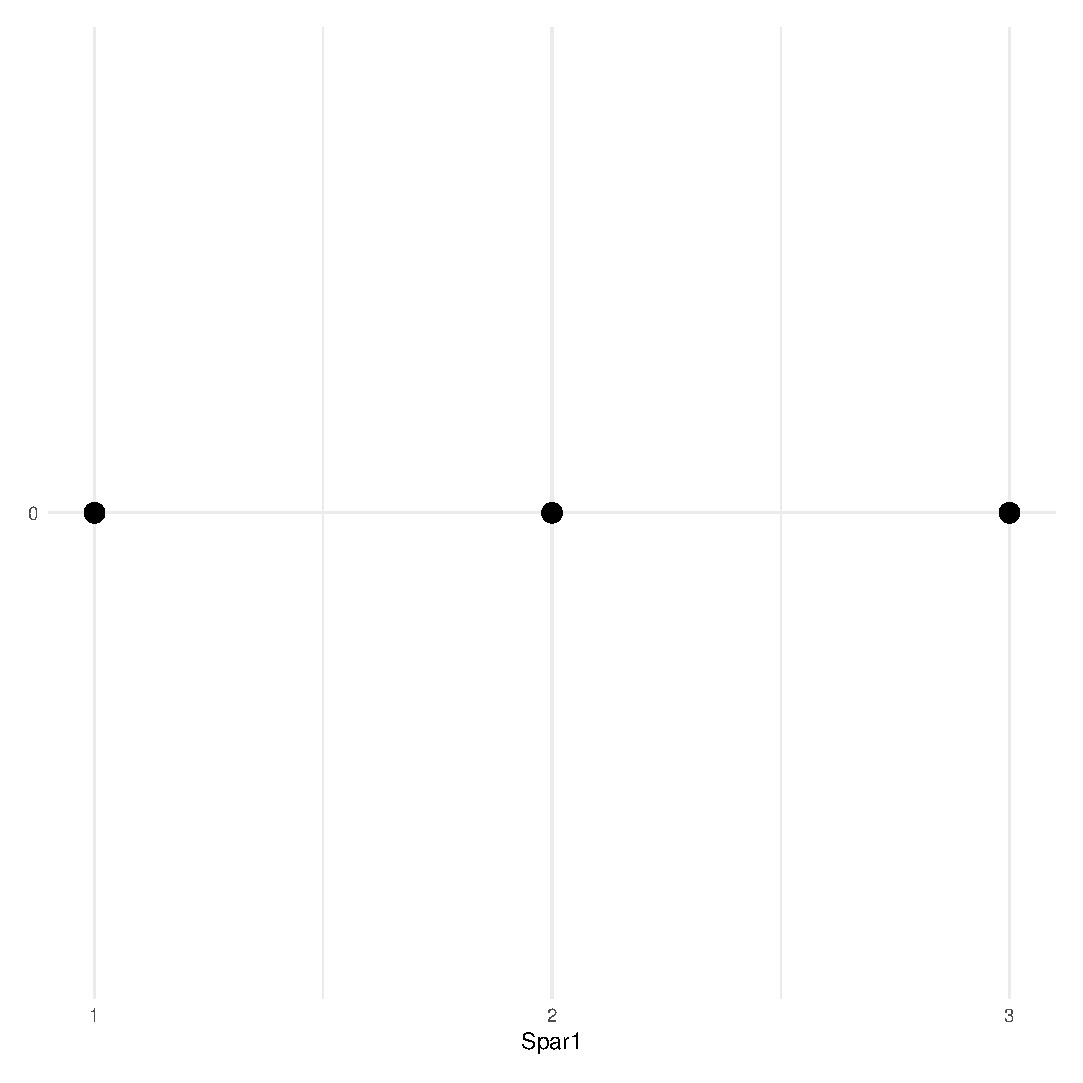
\includegraphics[width=0.9\textwidth]{../../images/points1}
  \end{minipage} %
  \begin{minipage}{0.45\textwidth}
    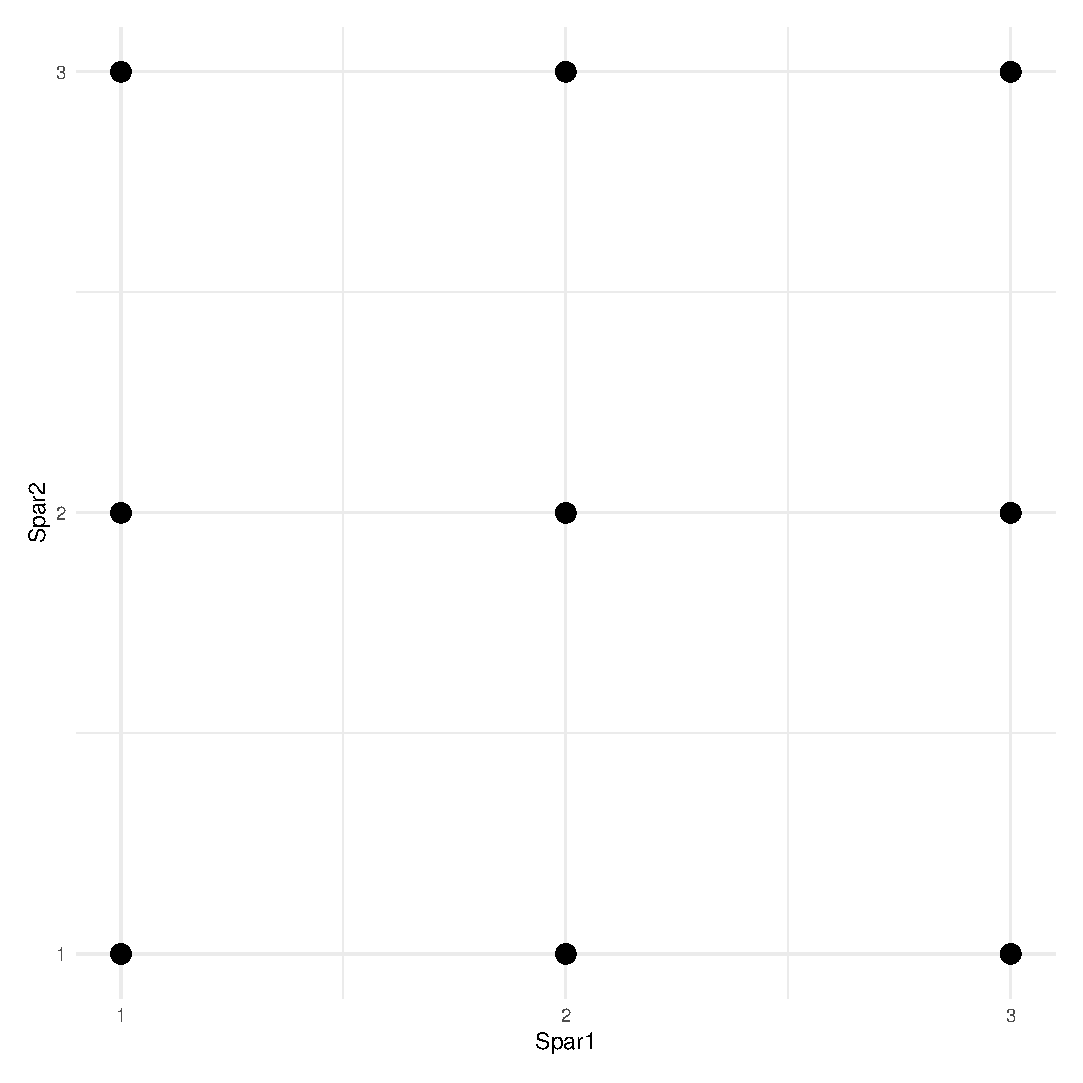
\includegraphics[width=0.9\textwidth]{../../images/points2}
  \end{minipage}
  \caption{Visual depiction of samples for $d=1$ and $d=2$.}
  \label{fig:samples}
\end{figure}

\emph{Exponential} scaling is bad, but some of the badness can be lost in
abstraction. If the one-dimensional case took $10$ seconds to execute, Table
\ref{tab:exponential} give execution times for some values of $d$. Note that by
$d=20$, the total execution time for our `simple' parameter study is already 240
times the age of the universe. Clearly, this is quite bad.

\begin{table}[!ht]
  \centering
  \begin{tabular}{r|r|l}
  \hline
  Dimension & Time (sec) & Comparison\\
  \hline
  1 & $10^{1}$ & Ten seconds\\
  \hline
  5 & $10^{5}$ & One Day\\
  \hline
  10 & $10^{10}$ & Eleven generations\\
  \hline
  18 & $10^{18}$ & Age of Universe\\
  \hline
  20 & $10^{20}$ & 230 x AoU\\
  \hline
  \end{tabular}
  \caption{Execution times for example parameter study. Punchline: exponential
    scaling is \emph{very, very bad}.}
  \label{tab:exponential}
\end{table}

This exponential scaling is one manifestation of \emph{the curse of
  dimensionality}.

\section{Curse of Dimensionality}
% --------------------------------------------------
The \textbf{curse of dimensionality}\footnote{Coined by Richard Bellman in the
  context of `exhaustive optimization'.} is the general phenomena of cost
scaling exponentially with dimension. This is actually a somewhat \emph{vague}
term, as dimensionality manifests differently across
contexts.\cite{donoho2000high} Some (academic) examples include:

\bigskip\noindent\underline{Integration:} Employing a tensor quadrature grid (as
visualized in Fig. \ref{fig:samples}) for quadrature directly leads to
exponential cost.

\bigskip\noindent\underline{Sampling:} Sampling according to a tensor design
leads to exponential cost. Note, however, that the Monte Carlo algorithm
(sampling from a density to approximate expectations) is \emph{not} cursed by
dimensionality, as Monte Carlo is dimension
independent.\cite{owen2013montecarlo}

\bigskip\noindent\underline{Machine Learning:} (Requirement of large data)

\bigskip\noindent\underline{Inference:} \textcolor{red}{TODO:}

\bigskip\noindent\underline{Distance:} \textcolor{red}{TODO:} Failure
of nearest neighbors.

\bigskip\noindent\underline{Big Data:} In 2000, David Donoho gave a talk on the
curse of dimensionality as it relates to data analysis.\cite{donoho2000high}
He noted that in industry,

\begin{quote}
  The trend today is towards more observations \emph{but even more so},
  \textcolor{palered}{to radically larger numbers of variables} – voracious,
  automatic, systematic collection of hyper-informative detail about each
  observed instance.\footnote{Emphasis mine}
\end{quote}

Statisticians usually consider data in terms of a matrix; with rows representing
$n$ observations, and columns representing $d$ variables. Dimensionality is thus
`one-half' of the bigness of data.

Hopefully one of the contexts above is relevant to you. Assuming this is the
case, then dimensionality is \emph{your} problem! We've seen one way
dimensionality affects a particular context (tensor-product sampling designs),
but why does dimensionality affect all these \emph{different} contexts? To build
some intuition, let's take a look at some properties of high-dimensional
geometry.

\subsection{High-Dimensional Geometry}
% -------------------------
Why is dimensionality so challenging? Here we talk about a few properties of
high-dimensional geometry. The intent is to (1) underscore that high-dimensional
spaces have `surprising' behavior, and (2) build some intuition for
dimensionality, with an aim towards challenges and potential solutions.

\subsubsection{Fact 1}
The hypersphere has vanishing interior.

\bigskip
In low dimensions, it can be easy to think of a uniform distribution -- really
just the volume of a solid -- as being `even' across the space. While this is
formally what a uniform distribution is, our geometric intuition for what that
means can start to break down in higher dimensions. As an example, let's
consider the volume integral for a unit \emph{hypersphere}; the set of all
points $\cH=\{\vx\in\R{d}\,|\,\|\vx\|\leq 1\}$, given in spherical coordinates
in \eqref{eq:hypersphere-volume}.

\begin{equation*} \begin{aligned} \label{eq:hypersphere-volume}
    HV &= \int\cdots\int \textcolor{red}{r^{d-1}}\,
         T(\varphi_{1},\dots,\varphi_{d-1})\,
         dr d\varphi_{1}\cdots d\varphi_{d-1}
\end{aligned} \end{equation*}

\noindent The integrand of \eqref{eq:hypersphere-volume} can be understood as a
sort of `volume density' -- the quantity we will integrate to compute the
volume. In areas where this integrand is large we see more volume contributed,
while in areas where this is small, relatively little volume is contributed.
Expressing this integral in spherical coordinates allows us to focus on how
volume contributions change along the radial coordinate $r$.

Note that the exponent in $r^{d-1}$ already points to some sort of `exponential
badness' we might expect from dimensionality. This factor in the integrand (Fig.
\ref{fig:hypervolume}) shows that the integrand tends to grow as one moves from
the origin towards the edge of the hypersphere. However, this growth becomes
distorted in higher dimensions; at $d=50$ the integrand is nearly zero until
about $r>0.9$, which means there is essentially no volume contributed until one
reaches the edge of the sphere. It is in this sense that we say the hypersphere
is empty.

\begin{figure}[!ht]
  \centering
  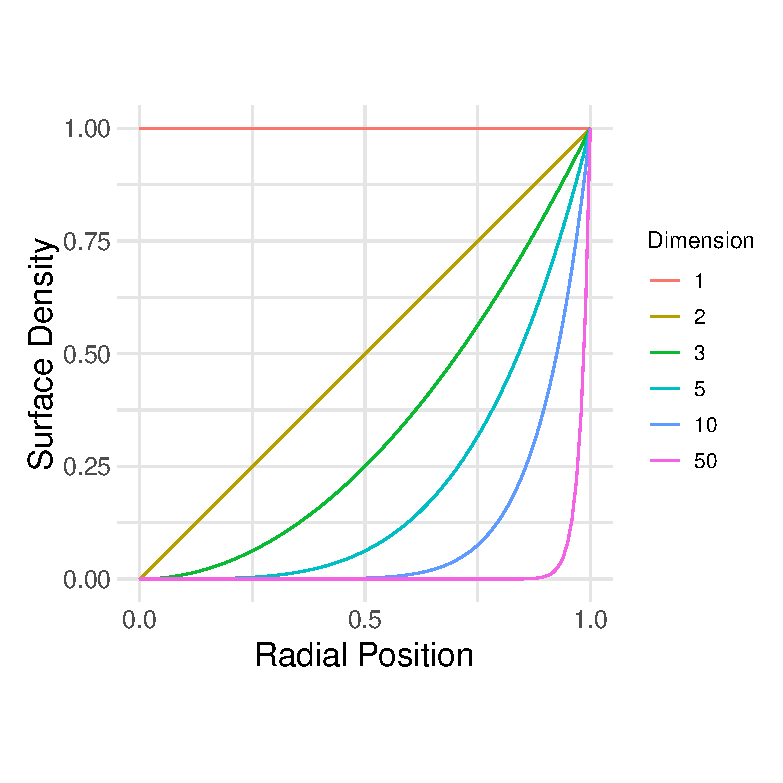
\includegraphics[width=0.65\textwidth]{../../images/surface_density}
  \caption{Radius-dependent portion of the integrand for a (unit) hypersphere
    volume calculation. Note that for higher dimensions, nearly all of the
    integrand is concentrated near the edge of $r=1$. This demonstrates that the
    hypersphere is empty -- that all of its volume is concentrated at its edge.}
  \label{fig:hypervolume}
\end{figure}

Practically, this means that if we sample uniformly from a hypersphere, then in
high dimensions, we will surely `miss' the interior. If our intent was to
understand the relation between input and response, then this is a region of a
function's input that we will not learn about. Depending on the context, this
may (or may not!) be an issue.

\clearpage
\subsubsection{Fact 2} All the volume in a hypersphere is near
\emph{the} equator.

\bigskip
Upfront, this is a bit of a wordgame; there are actually \emph{many} equators on
any sphere. On Earth, we define a single equator, but one can actually think of
an infinite family of equators, each enclosed by a great circle (Fig.
\ref{fig:great-circle}). These equators are formed by intersecting a
3-dimensional sphere (a `3-sphere') with a 2-dimensional plane that passes
through the sphere's origin, forming a 2-dimensional object. Since there are
infinitely many such planes, there are infinitely many equators.

\begin{figure}[!ht]
  \centering
  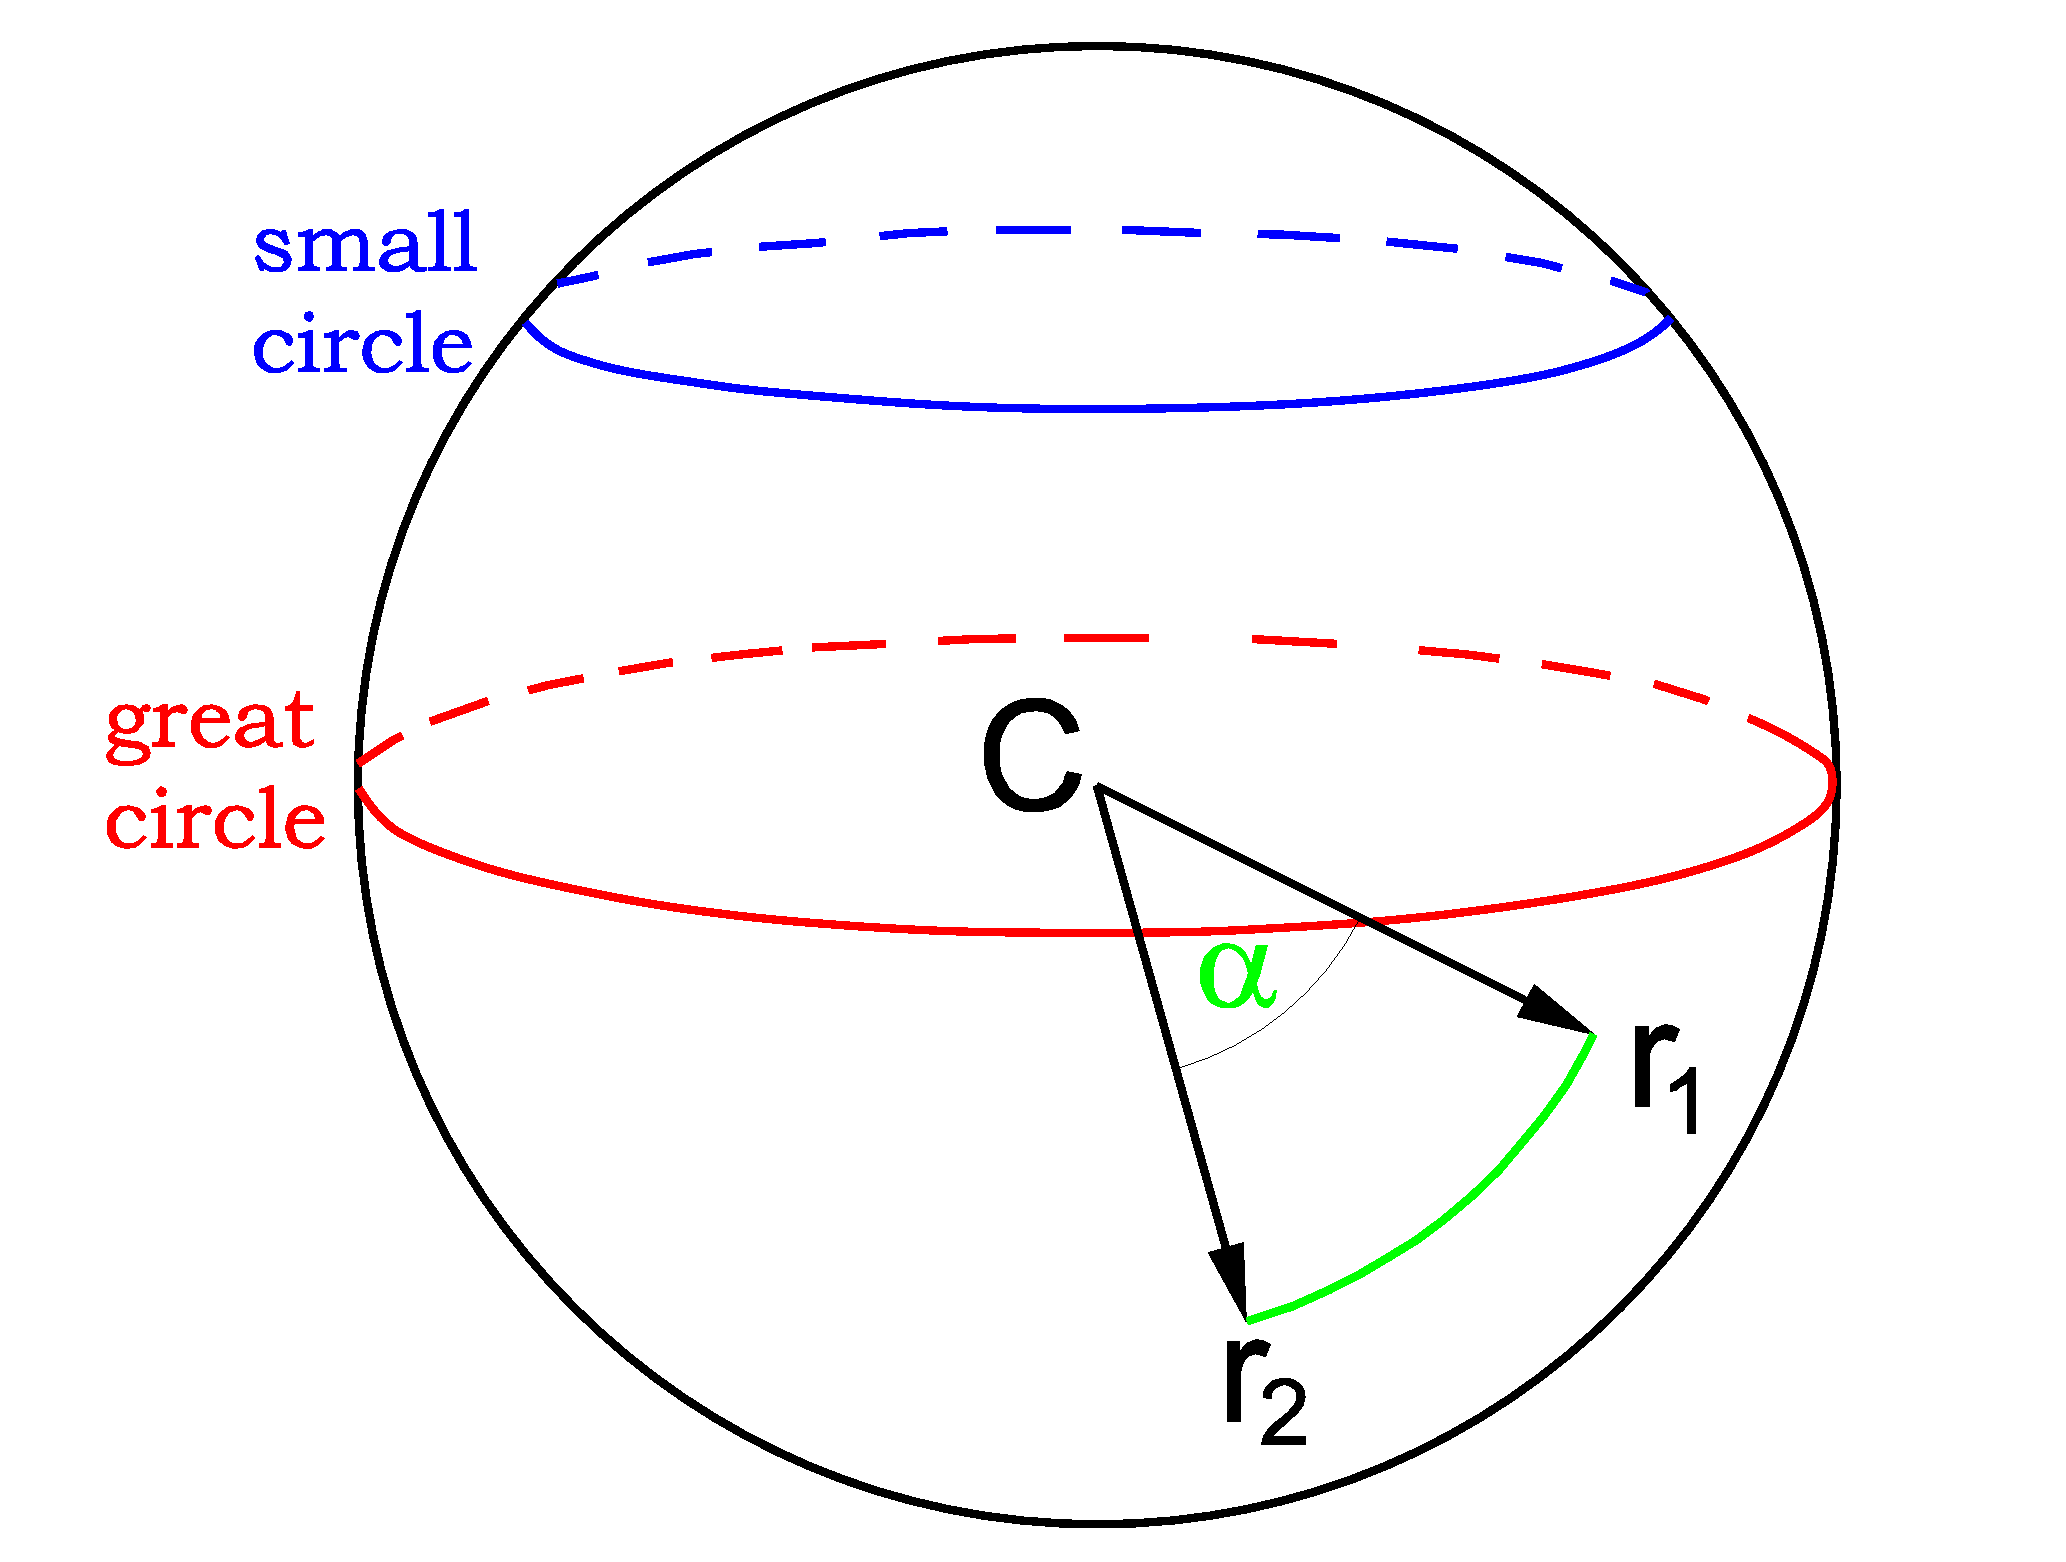
\includegraphics[width=0.65\textwidth]{../../images/great_circle}
  \caption{Cartoon depicting the boundary of a great circle for a 3-sphere. The
    red curve depicts a great circle; which encloses an equator. Thus, for the
    3-sphere, an equator is a 2-dimensional object. In higher dimensions $d$,
    the analog of an equator is a $d-1$-dimensional object. From Wikimedia
    Commons, CC P.wormer.}
  \label{fig:great-circle}
\end{figure}

In higher dimensions $d$, an equator is always a $d-1$-dimensional object. Thus,
as $d$ grows, an equator neglects proportionally less with regard to the full
dimensionality of the space. Thus, if we were to sample points uniform randomly
from within the $d$-dimensional sphere, this `neglected' dimension would
contribute less in higher dimensions. The result is that the volume -- which can
be linked to the uniform density in the hypersphere -- concentrates towards
\emph{any} chosen equator. We can see this by picking an arbitrary equator,
sampling at random, and computing the histogram of angles formed by the vector
between drawn points, the origin, and the chosen equator. Figure
\ref{fig:equator} shows results from this computer experiment: The realized
angles concentrate towards zero as $d$ increases.

\begin{figure}[!ht]
  \centering
  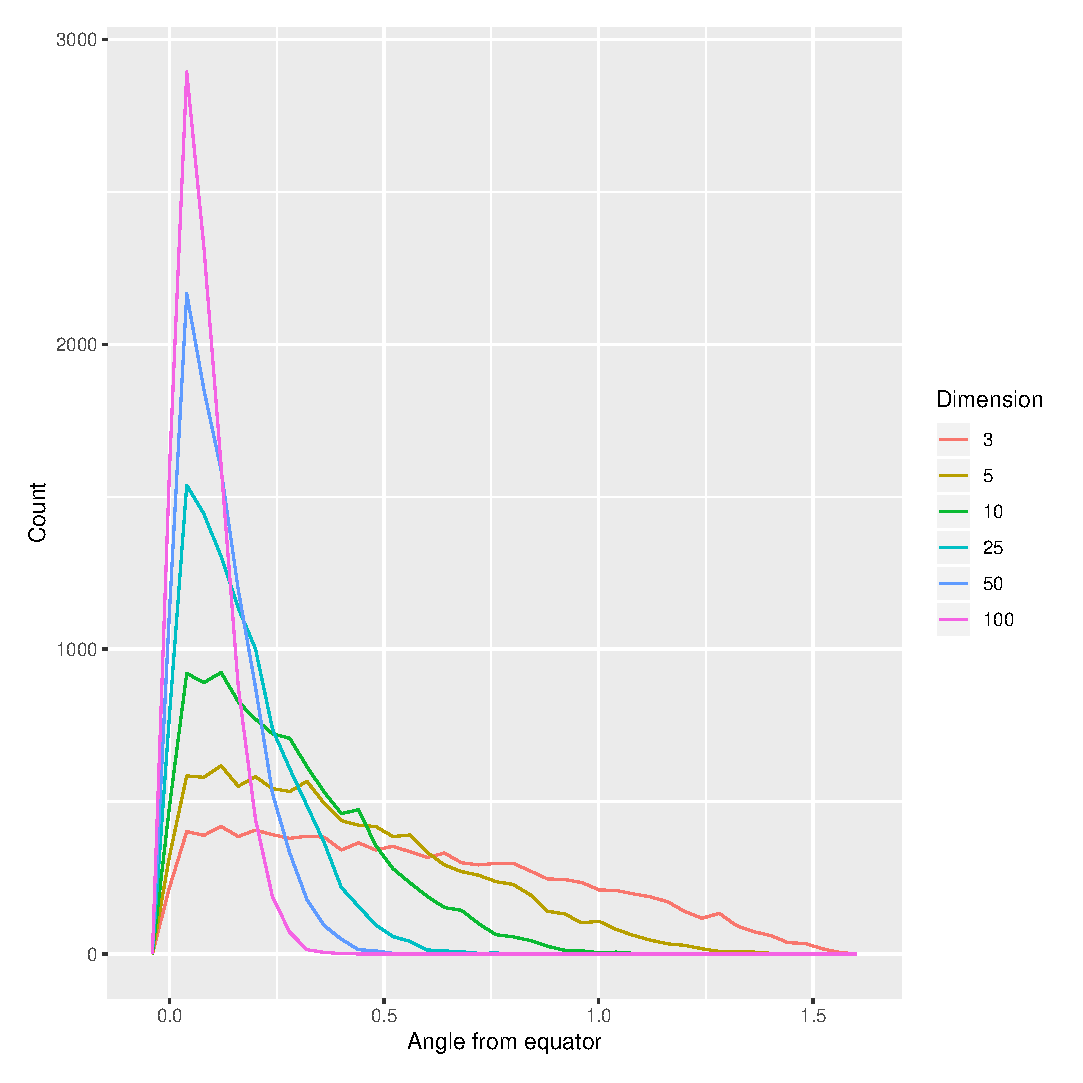
\includegraphics[width=0.65\textwidth]{../../images/equator}
  \caption{Realized angles away from a chosen equator for a $d$ dimensional
    hypersphere, estimated as empirical densities. This illustrates that, as
    $d\to\infty$, most points in the hypersphere (thus the volume) are
    concentrated near an equator.}
  \label{fig:equator}
\end{figure}

Similar to above, in high dimensions we will `miss' some \emph{directions} when
sampling uniformly from the hypersphere. As noted with Fact 1, this may or may
not be an issue, depending on the context.

Facts 1 and 2 really are pure geometric properties. I suspect that if we could
visualize higher-dimensional spaces, these `surprising facts' would be obvious.
The next fact relies on some properties\footnote{concentration of measure} of
random variables, and so relies on a bit more than geometry alone.

\clearpage
\subsubsection{Fact 3}
Random projections preserve pairwise distances.

\bigskip
First, we'll illustrate this fact with an example, then describe the theorem
that backs it up. I use some gene expression data from the UC Irvine machine
learning databse\cite{blake1998uci} for this example.\footnote{The specific data
  source is not terribly important here; the point is that the data are not
  `cooked' for demonstration purposes.} The data are loaded into the variable
\lstinline{mat_data}; the data have dimensions

\begin{lstlisting}
## Gene data from UCI
dim(mat_data)
#       Observations,  Dimensions
> [1]   801,           20531
\end{lstlisting}

We select a random projection of dimensionality \lstinline{k} via some
mysterious, to-be-described procedure, based on a user-selected error tolerance
\lstinline{eps}.

\begin{lstlisting}
## Make reproducible
set.seed(101)
## Calculate dimension
C <- 1                             # Over-samping factor
n <- dim(mat_data)[1]              # Observations
d <- dim(mat_data)[2]              # Dimensionality

k <- C * ceiling(log(n) / eps ^ 2) # J-L dimension
k
> 1338 (6.5% of 20531)
\end{lstlisting}

This mysterious procedure has suggested a projection of dimensionality $1338$,
just $6.5\%$ of $20531$.

A bonus fact is that, in high dimensions, random vectors drawn from an isotonic
gaussian\footnote{A gaussian possessing a diagonal covariance matrix} will
essentially be orthogonal.\cite{ailon2009fast} We can use this fact to easily
construct a random projection of the desired size.

\begin{lstlisting}
## Random `projection`
P <-
  rnorm(d * k, sd = 1 / d) %>%
  matrix(nrow = d, ncol = k)
## Project the data
mat_proj <-
  mat_data %*% P
\end{lstlisting}

When we project to a smaller dimensionality, we tend to decrease the average
distance between points. To have any hope of preserving pairwise distances, we'd
better account for this fact.

\begin{lstlisting}
## Match the original average distance; Subsample for speed
Ind <- sample(x = 1:n, size = 500)

D_sub_orig <-
  mat_data[Ind, ] %>%
  dist()

D_sub_fix <-
  mat_proj[Ind, ] %>%
  dist()

factor <-
  mean(D_sub_orig, na.rm = TRUE) / mean(D_sub_fix, na.rm = TRUE)

mat_proj <-
  mat_proj * factor
\end{lstlisting}

The claim is that the projected data \lstinline{mat_proj} possesses the same
pairwise distances $\|\vu-\vv\|$ as \lstinline{mat_data}, to within the chosen
tolerance \lstinline{eps}; let's check if that is the case.

\begin{lstlisting}
## Re-compute distances with proper scaling
Ind <- sample(x = 1:n, size = 500) # New draw

D_sub_orig <-
  mat_data[Ind, ] %>%
  dist()

D_sub_proj <-
  mat_proj[Ind, ] %>%
  dist()

## Compute quantiles of discrepancy
R_diff <- (D_sub_proj - D_sub_orig) / D_sub_orig
qt <- quantile(R_diff)
## qt
sprintf(
  "%5.3f%% %5.3f%% %5.3f%% %5.3f%% %5.3f%%",
  qt[1] * 100,
  qt[2] * 100,
  qt[3] * 100,
  qt[4] * 100,
  qt[5] * 100
)
>      0%     25%    50%    75%   100%
> -7.784% -1.193% 0.082% 1.344% 8.139%
\end{lstlisting}

In this case, the realized distortion is indeed within $\pm10\%$. This is a bit
mysterious -- by \emph{randomly} throwing out information, we were able to
preserve a great deal of structure in the data. The
\textbf{Johnson-Lindenstrauss lemma} (J-L) shows that this is no accident, but
rather a general property of high-dimensional spaces.

\bigskip
\underline{Lemma:} (Johnson-Lindenstrauss) For any $0<\epsilon<1$ and
$n\in\mathbb{Z}_{>0}$, let $k\in\mathbb{Z}_{>0}$ such that

\begin{equation} \label{eq:jl-bound}
  k \geq C \frac{\log(n)}{\epsilon^2},
\end{equation}

\noindent then for all sets of points $V\subset\R{d}$, there is a projection
$P_k:\R{d}\to\R{k}$ with $\alpha\in\R{}_{>0}$ such that, for all $u,v\in V$, we
have

\begin{equation} \label{eq:jl-distance}
  (1 - \epsilon)\|\vu - \vv\|^2 \leq \alpha\|P_k(\vu) - P_k(\vv)\|^2 \leq %
  (1 + \epsilon)\|\vu - \vv\|^2.
\end{equation}

\noindent Further, this projection can be found in polynomial time.

\bigskip
Numerous proofs of this statement\footnote{note that I've modified the statement
  above to emphasize certain elements, in the interest of aiding explanation.
  The `true' J-L lemma is stated slightly differently; I've made $\alpha$
  explicit in the statement above} exist, for an example see Dasgupta and
Gupta.\cite{dasgupta2003elementary}

Let's first try to understand the statement above. \Cref{eq:jl-distance} is a
statement about pairwise distances $\|\vu-\vv\|$ and their projected versions
$\|P_k(\vu) - P_k(\vv)\|$. J-L states that \emph{all} points in a given (data)
set satisfy this condition. Precisely, the projected pairwise distances can only
be distorted at most by a factor of $(1\pm\epsilon)$.

Note that the projected pairwise distances are multiplied by a positive value
$\alpha$. This is because projections reduce the \emph{average} distance between
points, as illustrated in Figure \ref{fig:jl-avg-distance}. If we want any hope
of matching pairwise distances, we have to account for this fact. I do this very
simply in the code above by computing $\alpha$ from the ratio of average
distances between the original and projected data -- we then restore by
multiplying by alpha.

\begin{figure}[!ht]
  \centering
  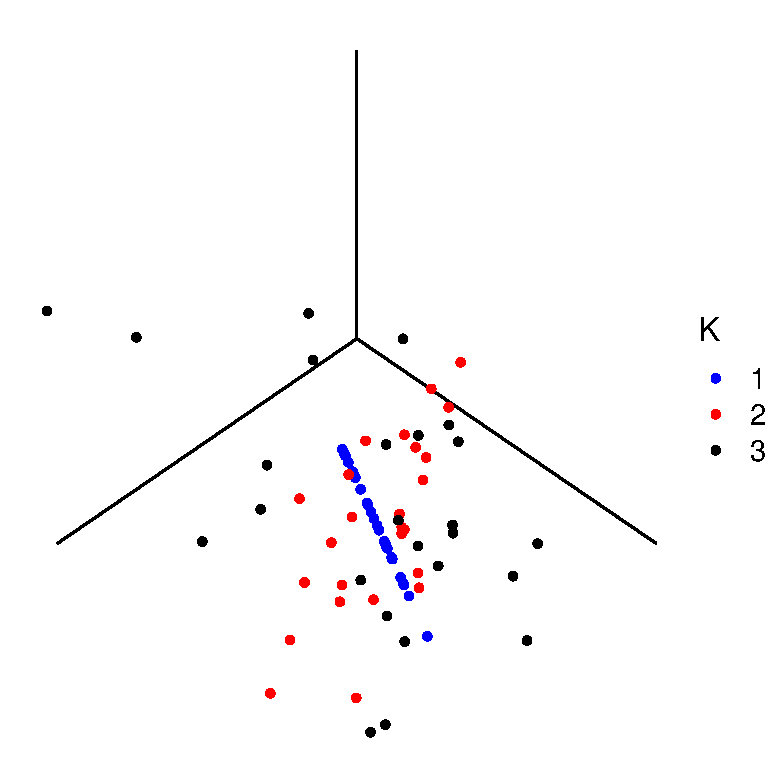
\includegraphics[width=0.65\textwidth]{../../images/dim_proj1}
  \caption{Example points in 3d space, projected to lower dimensions. Note the
    average distance between points is reduced with successively smaller
    projections. This is accounted for in \eqref{eq:jl-distance} by the $\alpha$
    factor, which corrects for these mean-distance effects.}
  \label{fig:jl-avg-distance}
\end{figure}

\Cref{eq:jl-bound} provides a target dimensionality based on provided
quantities. Provided the number of observations $n$ and desired error tolerance
$\epsilon$, J-L suggests a minimum projection dimension $k$. Note that
\emph{dimensionality is absent} from this bound. The original dimensionality $d$
can be arbitrarily large; given the same $n$ and $\epsilon$, the bound on
projection dimension will be the same.

This dimensionality $k$ is something we'll refer to -- in a somewhat
\emph{vague} sense -- as \emph{intrinsic dimensionality}. Within a space of
dimension $d$, there is low-dimensional structure of size $k$ (the mapping
$\alpha P_k(\cdot)$) that preserves information of interest, here pairwise
distances. This points forward to a general strategy for lifting the curse of
dimensionality -- if we can identify low-dimensional that preserves the
properties we care about, then we can reduce the effective dimensionality from
$d$ to $k$, and (potentially) render tractable the problems we want to solve.
This is the idea behind \emph{dimension reduction}.

\section{Dimension Reduction}
% --------------------------------------------------

\textbf{Dimension reduction} is the general strategy of identifying some form of
low-dimensional structure within a problem. Since there are many different
problem settings and objectives -- thus many \emph{kinds} of structure -- we
introduce a simple taxonomy to help distinguish different flavors of dimension
reduction.

\subsection{A Taxonomy}
% -------------------------
We will discuss three flavors of dimension reduction, broadly categorized by the
interpretation of $\R{d}$. Note that many of the techniques we will introduce
are applied across different contexts -- the mathematics does not appreciably
change in these different settings. However, the \emph{interpretation} of
mathematics changes across settings; if we seek to understand how the math
applies to our particular setting -- and if we seek to understand work by other
researchers in different fields -- then this difference in interpretation is
meaningful.

For instance, the singular value decomposition (SVD) shows up under different
names in different communities: the Karhunen-Loeve expansion (KLE), the proper
orthogonal decomposition (POD), principal component analysis (PCA), etc.
Mathematically, there is little difference between these ideas. However, a
person using the term KLE will generally be thinking of a different kind of
problem than someone speaking of PCA. Further, different properties of the SVD
are relevant in these different contexts. Both the communication aims and
technical details are conveyed by the different terminology.

We will describe the taxonomy of different settings, then focus on the
\emph{input-space} setting to give a bit more detail.

\bigskip\noindent A \underline{generic-space} is $\R{d}$ with no special
assumptions. Techniques like the Johnson-Lindenstrauss lemma and principal
component analysis\cite{fodor2002survey} are used in this context.

\bigskip\noindent An \underline{output-space} is $\R{d}$ understood as the
output of some (dynamical) system; the $d$ entries of a vector from $\R{d}$
could represent a time-varying signal (e.g. a speech sample), the pointwise
entries of some field (e.g. a mean channel-flow field), or some combination
(e.g. a time-varying flow field). The techniques of compressed sensing
(CS)\cite{candes2008introduction} and the proper orthogonal
decomposition\cite{lumley2007} are often used in this context.

\bigskip\noindent An \underline{input-space} is $\R{d}$ understood as the input
space to some function $f(\vx)$. Compressed sensing is also used in this
context,\cite{tang2014subsampled} but other approaches are a bit more common. We
will discuss these below, under additional broad categorizations.

\subsection{Input-space: Running Example}
% -------------------------
To explore input-space dimension reduction techniques, we first introduce the
simple illustrative problem of rough pipe flow, like that originally studied by
Osborne Reynolds.\cite{reynolds1883}

\begin{figure}[!ht]
  \centering
  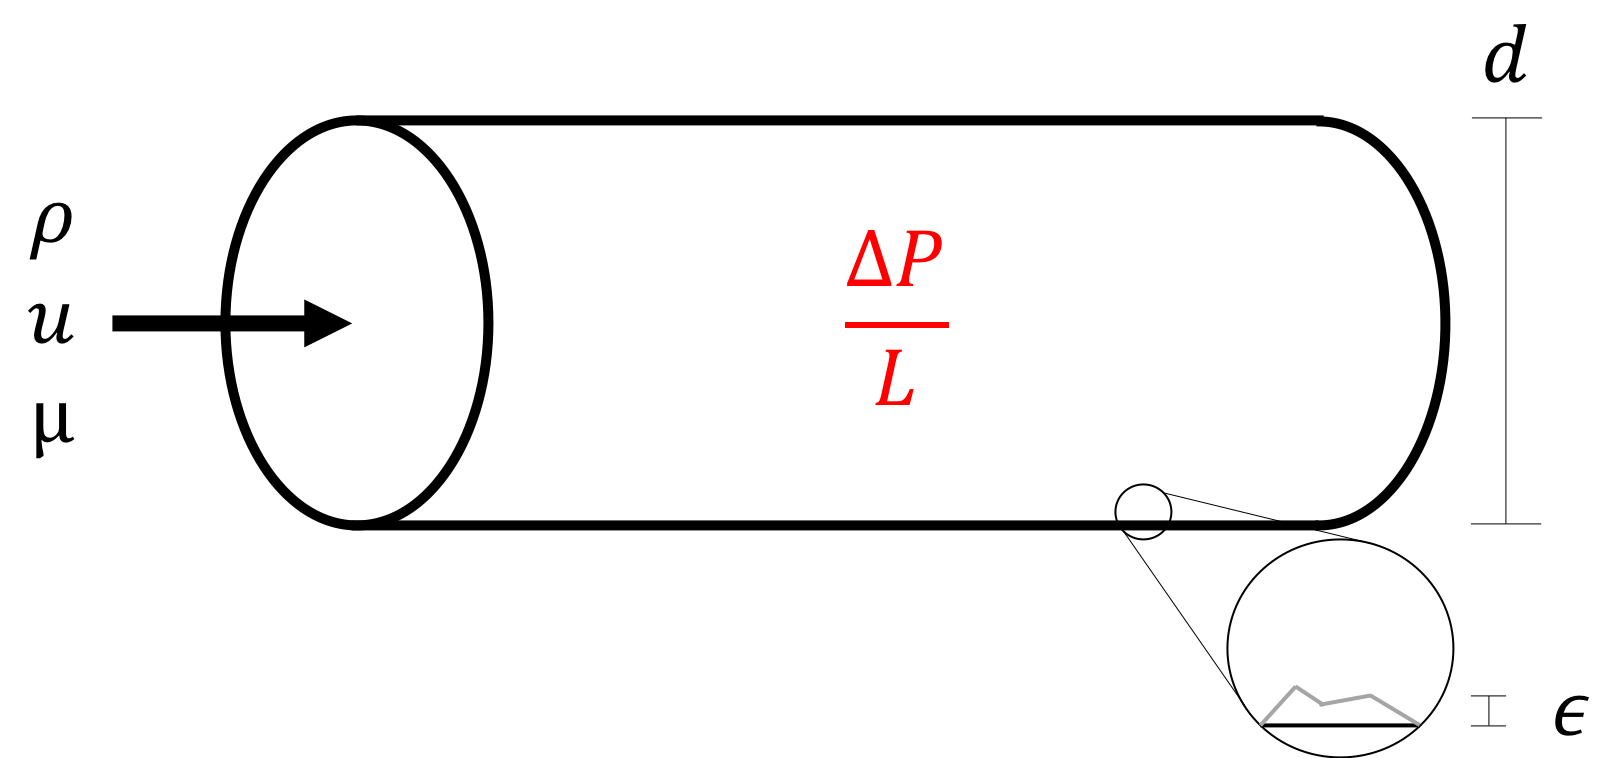
\includegraphics[width=0.65\textwidth]{../../images/pipe_diagram}
  \caption{Schematic for example pipe flow problem. A viscous fluid is pumped
    through a rough pipe. Our output quantity of interest is the (normalized)
    pressure loss -- a measure of the effort required to pump the fluid. The
    inputs are the fluid properties and pipe geometry.}
  \label{fig:pipe_diagram}
\end{figure}

We will categorize the following input-space reduction techniques into
\emph{subset reduction} and \emph{subspace reduction} approaches.

\subsection{Subset Reduction}
% -------------------------
When pursuing a \emph{subset reduction}, we aim to select a subset
$\{x_i\}_{i\in I}$ of the full set of variables $\{x_i\}_{i=1,\dots,d}$. The
rationale is as follows: Suppose our qoi had some complementary subsets of
\emph{active} $\{x_i\}_{i\in I_A}$ and \emph{inactive} $\{x_i\}_{i\in I_I}$
variables, such that $I_A\cup I_I = \{1,\dots,d\}$ and $I_A\cap
I_I=\varnothing$. Further suppose this split had the property that, for all
$x_i\neq x'_i$ with $i\in I_I$ and $x_j=x'_j$ with $j\in I_A$, we have

\begin{equation} \label{eq:inactive}
  f(\vx) = f(\vx').
\end{equation}

\noindent In words, the inactive variables do not contribute to changes in the
value of $f$. In this (admittedly contrived) setting, one can safely set the
inactive variables $\{x_i\}_{i\in I_I}$ to fixed, nominal values, and carry out
further studies on the active variables -- this reduces dimensionality to $k =
|I_A|$.\footnote{Where I use $|\cdot|$ to denote set cardinality.}

Of course, one can ask why these supposedly inactive variables were in the
function to start. Practically, the condition \eqref{eq:inactive} does not
frequently occur in practice; however, this condition is approximately met in
many practical applications. The precise definition of `approximately' results
in different subset reduction techniques. We will discuss two: Morris screening
and Sobol' indices.

\subsubsection{Morris screening}
\emph{Morris screening} can be thought of as studying contributions of variables
to the qoi through the mean and variance of the derivative. Ralph Smith's
textbook \cite{smith2013uncertainty} goes through this procedure in gory detail;
these notes will give only a brief introduction, as we'll focus more on Sobol'
indices. Morris screening considers statistics of the \emph{elementary effects},
defined by

\begin{equation}\label{eq:elem-effect}
  d_{i}(\vx_j) = \frac{f(\vx_j+\Delta \ve_i) - f(\vx_j)}{\Delta},
\end{equation}

\noindent where \(\ve_i\) is the i-th standard basis vector,\footnote{The vector with
all zeros, except for a one in the i-th entry} and \(\Delta\) is a large stepsize.
Note that \eqref{eq:elem-effect} is simply a first-order approximation of the
derivative; however, since \(\Delta\) is relatively large, this is a coarse
approximation to the derivative. These elementary effects are used to construct
global sensitivity measures

\begin{equation}\begin{aligned}
  \mu_i^* &= \frac{1}{r}\sum_{j=1}^r |d_{i}(\vx_j)|, \\
  \sigma_i^2 &= \frac{1}{r-1}\sum_{j=1}^r(d_{i}(\vx_j)-\mu_i)^2, \\
  \mu_i &= \frac{1}{r}\sum_{j=1}^rd_{i}(\vx_j).
\end{aligned}\end{equation}

This procedure is called \emph{screening} because it allows us to determine
whether individual parameters are unimportant, but does not quantify relative
variable importance. To determine relative importance, we can turn to Sobol'
indices. However, Morris screening is a relatively cheap procedure, and thus is
a good tool of which to be aware.

\subsubsection{Sobol' indices}
\emph{Sobol' indices} quantify importance of variables by attributing the
variance in the qoi to different inputs. They are a useful, well-studied, and
commonly-used technique for subset reduction, so we will spend some time
discussing them in detail: I learned this topic through the primer by Saltelli
et al.\cite{saltelli2004sensitivity}

Sobol' indices require a random variable interpretation of our quantity of
interest, so we'll introduce some notation used throughout the section. Let
\(\mX\sim\rho\) be our random input variables, distributed according to a joint
density \(\rho\) over our input space \(\Omega\).\footnote{Sobol' indices also
  have some properties that rely on independence of the inputs. We will return
  to this point later.} Then our output qoi is also a random variable
\(Y=f(\mX)\). We denote by \(\E[Y] = \int f(\vx)\rho(\vx)d\vx\) the expectation,
and by \(\V[Y]=\E[(Y-\E[Y])^2]\) the variance. Note that the following useful
identity involving the variance holds

\begin{equation}
  \V[Y] = \E[Y^2] - \E[Y]^2.
\end{equation}

We denote conditioning by a vertical bar; this corresponds to holding particular
random inputs fixed in value, and leaving them out of the integral for a
particular expectation. For example, if \(Y=f(X_1,X_2,X_3)\), then

\begin{equation}
  \E_{X_2,X_3}[Y|X_1=x_1] = \int f(x_1,x_2,x_3)\rho(x_1,x_2,x_3)dx_2dx_2,
\end{equation}

\noindent where we use subscripts to make explicit the integration variables.
Note that \(\E_{X_2,X_3}[Y|X_1]\) is still a random variable\footnote{when it
  lacks the equality \(X_1=x_1\)}, due to the variability arising from \(X_1\).
We will use conditional variance to decompose the total variance \(\V[Y]\)
according to different input contributions. This will involve expressions of the
sort \(\E_{X_2,X_2}[\V_{X_1}[Y|X_1]]\).\footnote{which is no longer a random
  variable, as we have integrated out all of the variables}

In what follows, we will drop the variable subscripts, as they tend to render
expressions indecipherable. The same information is implied by the conditioning;
the expression \(\V[Y|X_1]\) carries out the integration keeping \(X_1\) fixed,
which is then integrated out in the expression \(\E[\V[Y|X_1]]\).

To construct the Sobol' indices, we will derive a particular variance
decomposition. First, we will introduce some notation to help keep track of
variable subsets. Let \(\vu\) be an \emph{index set}; that is
\(\vu\subseteq\{1,\dots,d\}\). We will use \(\vu\) to denote subsets of the
input variables; in the example above, we used \(\vu=\{2,3\}\) to give us
\(\mX_{\vu}=\{X_2,X_3\}\). Let \(-\vu\) be the set complementary to \(\vu\) with
respect to \(\{1,\dots,d\}\); in the example above \(-\vu=\{1\}\).

Next, we will prove a simple identity, which will allow us to attribute the
variance \(\V[Y]\) to different inputs. Note that for any index set \(\vu\), we have

\begin{equation}\begin{aligned}\label{eq:var-decomp}
  \E[\V[Y|\mX_{\vu}]] + \V[\E[Y|\mX_{\vu}]] &= %
  \E[\E[Y^2|\mX_{\vu}] - \cancel{ \E[Y|\mX_{\vu}]^2 }] \\
  &+ \cancel{\E[\E[Y|\mX_{\vu}]^2]} - \E[\E[Y|\mX_{\vu}]]^2, \\
  &= \E[Y^2] - \E[Y]^2, \\
  &= \V[Y^2].
\end{aligned}\end{equation}

\noindent \Cref{eq:var-decomp} allows us to decompose the variance into two
terms that we can interpret. First, note that the expression
\(\V[\E[Y|X_{\vu}]]\) first averages out all the variables \(\mX_{-\vu}\), then
computes the variance due only to \(\mX_{\vu}\). We may use this expression with
a singleton index set \(\vu=\{i\}\) to define the \emph{first-order sensitivity
  index}

\begin{equation}\label{eq:sobol-first}
  \underline{\tau}_{\{i\}}^2 = \frac{\V[\E[Y|X_i]]}{\V[Y]}.
\end{equation}

\noindent \Cref{eq:sobol-first} is bounded between \([0,1]\), and enables us to
rank variables according to their importance. Practically
\(\underline{\tau}_{\{i\}}^2\) tells us how much variance reduction we could
expect if we were able to exactly freeze \(\mX_i\). We could use this information
to inform which variables we should better characterize, in order to reduce
variability.

Note that we should not use \(\underline{\tau}_{\{i\}}^2\) to perform dimension
reduction; the first-order index does not account for interactions with other
variables, so we may miss some important cross terms. Instead, we may consider
the \emph{total-order sensitivity index}

\begin{equation}\label{eq:sobol-total}
  \overline{\tau}_{\{i\}}^2 = \frac{\E[\V[Y|X_{-\{i\}}]]}{\V[Y]} = %
  1 - \frac{\V[\E[Y|X_{-\{i\}}]]}{\V[Y]}.
\end{equation}

\noindent \Cref{eq:sobol-total} is also bounded between \([0,1]\), and accounts
for interactions between \(X_i\) and all other variables. We may interpret
\eqref{eq:sobol-total} in at least two ways: As the variability in \(Y\) due to
\(X_i\), averaged over all other inputs (middle expression), or as the complement
of the variability arising from all the variables excluding \(X_i\) (right
expression). If \(\overline{\tau}_{\{i\}}^2\) is zero or small, we can be
confident that \(X_i\) contributes little to the variablility in \(Y\), neither
through first-order nor interaction effects.

In summary: The notation for the sensitivity indices is suggestive of their use.
The first-order index \(\underline{\tau}_{\{i\}}^2\) can be thought of as a
lower bound; if it is large, then we can be confident that \(X_i\) is important.
In contrast the total-order index \(\overline{\tau}_{\{i\}}^2\) is an upper
bound; if it is small, then we can be confident that \(X_i\) is unimportant.

Now an example of a Sobol' index computation: A very common test case for
demonstrating Sobol' indices is the so-called \emph{Ishigami
  function},\cite{ishigami1990importance} given in \eqref{eq:ishigami}.

\begin{equation*} \begin{aligned} \label{eq:ishigami}
  f(\vx) &= \sin(x_1) + 7\sin^2(x_2) + 0.1 x_3^4\sin(x_1) \\
  x_1, x_2, x_3 &\sim U[-\pi, \pi], \\
  \underline{\tau}_{\{3\}}^2 &= 0\%, \\
  \overline{\tau}_{\{3\}}^2 &= 24.4\%
\end{aligned} \end{equation*}

\noindent Above, Sobol' indices for $x_3$ are reported; note that $x_3$ enters
as a scaling factor on $\sin(x_1)$. The first-order Sobol' index for $x_3$
indicates that this variable is unimportant in a first-order sense; this is
because we first average over all other variables ($\sin(\cdot)$ averages to
zero as it is anti-symmetric) before computing the variance contributed. The
total-order index tells a different story -- here $x_3$ contributes
$\approx24\%$ of the total variance, in cooperation with the other inputs. This
example helps to drive home why total-order indices should be used for dimension
reduction.

What would we get for total Sobol' indices on the pipe flow problem? The results
Table \ref{tab:pipe-sobol} suggest that the roughness lengthscale $\epsilon$
alone is sufficient to capture the vast majority of variance in the output qoi.

\begin{table}[!ht]
  \centering
  \begin{tabular}{@{}llllll@{}}
   & $\rho$ & $U$ & $d$ & $\mu$ & $\epsilon$\\
  \hline
  $\V[f]$ & 0\% & 0\% & 6\% & 0\% & 94\% \\
  \end{tabular}
  \caption{Total Sobol' indices for pipe flow problem. The results suggest that,
    for capturing variance in $f$, the roughness $\epsilon$ alone is essentially
    the only relevant variable. Of course, this pre-supposes that variance is
    the `correct' measure to consider. The distributions for the inputs are
    chosen such that fully turbulent flow conditions are emphasized; this
    accounts for why roughness dominates in this setting.}
  \label{tab:pipe-sobol}
\end{table}

Sobol' indices seem to be useful for dimension reduction, but let's consider
their computational expense for a moment. Recall that Sobol' indices are defined
in terms of variance in the output qoi. Variance is defined in terms of an
expectation. Expectations are subject to the curse of dimensionality.

So is Sobol' itself cursed by dimensionality?



\subsection{Subspace Reduction}
% -------------------------
\textbf{Principal component analysis} \textcolor{red}{TODO:} PCA introduction

We can think of the \textbf{active subspace} as an object arising from a PCA on
gradient data; in fact, an early formulation of the active subspace was exactly
posed as such.\cite{russi2010uncertainty}

\textcolor{red}{TODO:} Active subspace tutorial

\textcolor{red}{TODO:} Active subspace example

\section{Intrinsic Dimensionality}
% --------------------------------------------------

\textcolor{red}{TODO:} vague concepts

\textcolor{red}{TODO:} Buckingham pi

\bibliographystyle{plain}
\bibliography{bibtex_database}

\end{document}
